%%%%%%%%%%%%%%%%%%%%%%%%%%%%%%%%%%%%%%%%%%%%%%%%%%%%%%%%%%%%%%%%%%%%%%%%%%%%%%%%
% Preámbulo                                                                    %
%%%%%%%%%%%%%%%%%%%%%%%%%%%%%%%%%%%%%%%%%%%%%%%%%%%%%%%%%%%%%%%%%%%%%%%%%%%%%%%%

\documentclass[11pt,a4paper,titlepage,oneside]{report}

%%% RELACIÓN DE VARIABLES A PERSONALIZAR %%%
\def\lingua{gal}
%\def\lingua{esp} % descomenta esta liña se redactarás a memoria en español
%\def\lingua{eng} % descomenta esta liña se redactarás a memoria en inglés
\def\nome{Brais Gómez Espiñeira}                             % substitúe aquí o teu nome
\def\nomedirectorA{José Manuel Vazquez Naya}              % substitúe aquí o nome de quen dirixe
%\def\nomedirectorB{Outro Nome Completo}             % duplica esta liña máis veces se o precisas, cambiando
                                                     % a letra final (A, B, C, D...): úsanse na portada.tex
\def\titulo{Open-source Secure NFC-based Physical Access Control System} % substitúe aquí o título do teu TFG
%\def\titulacion{gced}                               % descomenta esta liña e comenta a seguinte se es estudante do GCED
\def\titulacion{gei}
%\def\mencion{COMPUTACIÓN}                           % descomenta a mención que che corresponda se es estudante do GEI
\def\mencion{ENXEÑARÍA DO SOFTWARE}
%\def\mencion{ENXEÑARÍA DE COMPUTADORES}
%\def\mencion{SISTEMAS DE INFORMACIÓN}
%\def\mencion{TECNOLOXÍAS DA INFORMACIÓN}

%\def\renomearcadros{si} % descomenta esta liña se redactas a memoria en español e prefires que
                         % os "cuadros" e o "índice de cuadros" se renomeen
                         % a "tablas" e "índice de tablas" respectivamente

\usepackage{estilo_tfg}

% Lista de paquetes potencialmente interesantes (uso baixo demanda)
\usepackage{multirow}

\usepackage{hyperref}
% \usepackage{alltt}       % proporciona o entorno alltt, semellante a verbatim pero que respecta comandos
% \usepackage{enumitem}    % permite personalizar os entornos de lista
% \usepackage{eurofont}    % proporciona o comando \euro
% \usepackage{float}       % permite máis opcións para controlar obxectos flotantes (táboas, figuras)
% \usepackage{hhline}      % permite personalizar as liñas horizontais en arrays e táboas
  \usepackage{longtable}   % permite construir táboas que ocupan máis dunha páxina
% \usepackage{lscape}      % permite colocar partes do documento en orientación apaisada
% \usepackage{moreverb}    % permite personalizar o entorno verbatim
% \usepackage{multirow}    % permite crear celdas que ocupan varias filas da mesma táboa
% \usepackage{pdfpages}    % permite insertar ficheiros en PDF no documento
% \usepackage{rotating}    % permite diferentes tipos de rotacións para figuras e táboas
% \usepackage{subcaption}  % permite a inclusión de varias subfiguras nunha figura
% \usepackage{tabu}        % permite táboas flexibles
% \usepackage{tabularx}    % permite táboas con columnas de anchura determinada
\usepackage{float}
\usepackage{graphicx}
\usepackage{caption}

%%%%%%%%%%%%%%%%%%%%%%%%%%%%%%%%%%%%%%%%%%%%%%%%%%%%%%%%%%%%%%%%%%%%%%%%%%%%%%%%
% Corpo                                                                        %
%%%%%%%%%%%%%%%%%%%%%%%%%%%%%%%%%%%%%%%%%%%%%%%%%%%%%%%%%%%%%%%%%%%%%%%%%%%%%%%%

\begin{document}

 %%%%%%%%%%%%%%%%%%%%%%%%%%%%%%%%%%%%%%%%
 % Preliminares do documento            %
 %%%%%%%%%%%%%%%%%%%%%%%%%%%%%%%%%%%%%%%%

 \begin{titlepage}
  
  \hspace*{128pt}
  \textcolor{udcpink}{{\fontencoding{T1}\fontfamily{phv}\selectfont Facultade de Informática}}\\[-32pt]

  \begin{center}
    
\includegraphics[scale=0.3]{imaxes/udc}\\[25pt]

    {\large TRABALLO FIN DE GRAO \\
            \nometitulacion \\
            \nomemencion } \\[10pt]

    \carimbo \\[25pt]

    \begin{huge}
      \begin{spacing}{1.3}
        \bfseries \titulo
      \end{spacing}
    \end{huge}
  \end{center}
  
  \vfill
  
  \begin{flushright}
    {\large
    \begin{tabular}{ll}
      {\bf Estudante:} & \nome \\
      {\bf Dirección:} & \nomedirectorA \\
%                      & \nomedirectorB \\ % duplica esta liña máis veces se o precisas, cambiando
                                           % a letra final (A, B, C, D...); define eses nomes no memoria_tfg.tex
    \end{tabular}}
  \end{flushright}
  \rightline{A Coruña, \datasimple.}
\end{titlepage}

 \dedicatoria{A mi familia.} % escribe neste comando o teu texto de dedicatoria
 \paxinaenbranco
 \begin{agradecementos}
Thanks to my family and friends for supporting me.Also I want to thank José, Martiño and Rubén for their tutoring and guiding in order to complete this project. Furthermore, I want to thank my partners who always were friendly and helpful and the Citic Research department for financing this project.                % substitúe este comando polo teu texto de agradecementos
 \end{agradecementos}
 %%%%%%%%%%%%%%%%%%%%%%%%%%%%%%%%%%%%%%%%%%%%%%%%%%%%%%%%%%%%%%%%%%%%%%%%%%%%%%%%

\pagestyle{empty}
\begin{abstract}
  En la actualidad, el control de acceso físico está dominado por soluciones privadas y patentadas que son cerradas, inflexibles y a menudo inseguras. Para subsanar estas deficiencias, esta tesis presenta un sistema de control de accesos NFC de código abierto, modular y seguro. Soporta políticas basadas en el tiempo y en roles, permitiendo a los administradores proteger múltiples zonas dentro de la misma instalación desde un servidor de gestión centralizado.
  \par\vspace*{25pt}
  \begin{segundoresumo}
    Physical access control today is dominated by private, proprietary solutions that are closed, inflexible and often insecure. To address these shortcomings, this thesis presentsan open source, modular and secure NFC access control system. It supports time-based and role-based policies, enabling administrators to protect multiple zones within the same facility from a centralized management server.
  \end{segundoresumo}
\vspace*{25pt}
\begin{multicols}{2}
	\begin{description}
	\item [\palabraschavesecundaria:] \mbox{} \\[-20pt]
		\begin{itemize}
				\item NFC
				\item Access control
				\item Mutual authentication
				\item HSM module
		\end{itemize}
	\end{description}
	
	\begin{description}
	\item [\palabraschaveprincipal:] \mbox{} \\[-20pt]
		\begin{itemize}
			\item NFC
			\item Control de acceso
			\item Autenticación mutua
			\item Módulo HSM
		
		\end{itemize}
	\end{description}
\end{multicols}


\end{abstract}
\pagestyle{fancy}

%%%%%%%%%%%%%%%%%%%%%%%%%%%%%%%%%%%%%%%%%%%%%%%%%%%%%%%%%%%%%%%%%%%%%%%%%%%%%%%%


 \pagenumbering{roman}
 \setcounter{page}{1}
 \bstctlcite{IEEEexample:BSTcontrol}

 \tableofcontents
 \listoffigures
 \listoftables
 \clearpage
 
 \pagenumbering{arabic}
 \setcounter{page}{1}

 %%%%%%%%%%%%%%%%%%%%%%%%%%%%%%%%%%%%%%%%
 % Capítulos                            %
 %%%%%%%%%%%%%%%%%%%%%%%%%%%%%%%%%%%%%%%%

 \chapter{Introduction}
\label{chap:introduction}
Access Control is about controlling who can access a resource, either a physical building, a digital computer system or sensitive data. In the context of physical facilities, such as corporate offices, data centers, laboratories or manufacturing plants, access control systems integrate hardware (e.g. electromagnetic locks, microcontrollers or NFC/RFID readers) and centralized management software to enforce entry rules and audit log events into their solutions. By defining roles, schedules and zones of authorization, these solutions ensure that only properly credentialed individuals enter the right areas at the right times, reducing unauthorized entry, tailgating and insider threats \cite{Ref1}.

Over the past decade, advancements in wireless communication standards have driven the adoption of contactless technologies in security‑critical environments. Among these, Near Field Communication (NFC) stands out for its global standardization (ISO/IEC 14443)~\cite{Ref23}, interoperability with billions of mobile devices, and inherently short communication range, which mitigates relay‑attack risks \cite{Ref73}.

In the domain of access control, NFC has proven particularly effective, offering a balance between usability and security~\cite{Ref72}. Its contactless nature allows for rapid authentication at entry points, such as door access systems in offices or public transportation fare systems, where speed and convenience are critical. Also, NFC systems can be easily integrated with smartphones, enabling secure mobile payments and access control through applications, while also supporting robust encryption methods to safeguard transmitted data. It operates by leveraging tags or cards embedded with unique identifiers and cryptographic keys. These credentials are read by NFC-enabled devices to verify access rights in real time. Despite its advantages, NFC-based access control faces significant challenges, including the risks of cloning, unauthorized interception, and tampering~\cite{Ref2}.

However, most of the systems still employ basic cards such as MIFARE Classic~\cite{Ref28}, whose security is based on a set of static, reversible keys that can be extracted with low-cost hardware tools. These cards have been subject to multiple practical attacks after the release of their proprietary algorithms more than a decade ago~\cite{Ref79}. As a result, they remain vulnerable to spoofing and data manipulation, forcing today's migration to more robust technologies (e.g., NTAG 424 DNA with AES-128 and HMAC-SHA256) to ensure integrity and confidentiality in critical access control systems.

The growing demand for NFC physical access control solutions has been met with a lack of open and affordable alternatives~\cite{Ref3}. Most traditional access control systems rely on proprietary hardware such as RFID/NFC card readers, central management servers, and closed-source software platforms provided by commercial vendors. These solutions come from private companies such as HID Global~\cite{Ref4}, leader in the sector, whose complete implementations cost over 5,000\,€, and others such as Suprema~\cite{Ref5} or Honeywell~\cite{Ref6}. The pricing of these solutions is usually not affordable for Small and Medium-sized Enterprises (SMEs) and private users. In addition, these platforms tend to be closed and not very customizable. For example, HID SEOS\textregistered~\cite{Ref7}, despite its cryptographic robustness and cross-platform support, does not allow credentials to be generated or integrated into third-party environments without proprietary tools and licenses. While many vendors provide turnkey NFC‑based door controllers, these typically lock customers into proprietary ecosystems with high per‑unit costs. Moreover, closed APIs and opaque credential‑management workflows hinder integration with custom identity‑management platforms. This approach makes the system expensive and limits its flexibility~\cite{Ref74}.

This degree thesis project develops a modular, open-source, and cost-effective physical access control system using NFC. Motivated by the lack of affordable transparent solutions and the potential of NFC technology for securing physical facility entry, the developed system uses NFC cards, readers, and a web server to securely manage electronic locks and record entry events in real time. System administrators are able to configure user profiles, apply time-based permissions and centrally view a detailed access history through a web dashboard. In addition, the solution incorporates advanced cryptographic mechanisms (e.g., NTAG424, TLS or AES-128) to mitigate threats such as card cloning, unauthorized interception and data tampering. Furthermore, regarding the physical layer, the system leverages a microcontroller integrated with dedicated hardware modules, specifically designed for seamless interaction with NFC tags and secure communication with the web server.

\clearpage
\section{Objectives}
\label{sec:objectives}


The main objective of this work is to develop a modular, open source, cost-effective access control system using NFC technology to securely manage electronic locks and record entry events in real time.

The specific objectives are the following:
\begin{itemize}
	\item Analyze the technologies that are being used in the field of access control and identify the main security issues.
	\item Analyze the system requirements, design the system architecture, the protocol operation and the key management system.
	\item Develop and validate a working prototype using an iterative design approach, in which essential hardware components are progressively integrated until a complete access control system is achieved.
	\item Secure the communication between the different modules and implement security measures to avoid the main threats faced by NFC-based access control systems (e.g., data leaks, card cloning or impersonation).
	\item Develop a role-based web-based management system that allows the assignment and configuration of time-dependent access permissions, enabling administrators to precisely define authorized entry intervals for each user profile.
	\item Integrate a real-time alert mechanism that notifies administrators of access attempts outside predefined schedules, thus ensuring effective control and increased security in the access control system.
\end{itemize}


 \chapter{Background}
\label{chap:background}

This chapter outlines the fundamental concepts and technologies that underpin the system's design and implementation. It includes an overview of the hardware platforms used for embedded development, the cryptographic mechanisms for securing data, the principles of NFC communication, and the prototyping and communication protocols that enable interaction between components.

\section{Embedded Hardware and Development Environment}
\label{sec:embedded_hw}

The objective of this section is to describe the embedded platforms used for the development of the prototype. These solutions provide an accessible programming environment and a large support community, which facilitates iterative hardware implementation and the incorporation of specialized libraries.

\subsection{Arduino}
\label{subsec:arduino}
Arduino is an open-source software and hardware platform based on a board that includes electronic circuits with analog and digital inputs and outputs.  
The first Arduino board was introduced in 2005, and its popularity has not yet started to decrease.

One of the main reasons for this reputation is the wide number of modules it is compatible with, which leads to great flexibility in educational projects related to robotics and automation.

Arduino boards are small, low-power consuming computers. As shown in Figure~\ref{fig:arduino}, they have several components with different functionalities~\cite{Ref8}:

\begin{itemize}
	\item \textbf{Microcontroller:} receives and sends information to the devices connected to it. The specific chip depends on the board model.
	\item \textbf{External power supply:} powers the microcontroller with a DC voltage range of 9--12V.
	\item \textbf{USB plug:} used to upload code to the microcontroller through a USB cable. It can also supply 5V DC in absence of external power.
	\item \textbf{Internal programmer}
	\item \textbf{Reset button}
	\item \textbf{Analog pins:} used for analog input/output. Quantity varies between models.
	\item \textbf{Digital pins:} used for digital input/output. Quantity also varies.
	\item \textbf{Power and GND pins:} provide 3.3V, 5V and ground connections.
\end{itemize}
The board used in this project is an \textit{Arduino Uno}, which uses an ATmega328 microcontroller, has a clock speed of 16\,MHz with auto-reset, 14 digital I/O pins, 6 analog inputs, USB-B connection, and 32\,KB flash memory.  
The key feature regarding the selection of this board was the wide documentation available online~\cite{Ref9}.

\begin{figure}[h!]
	\centering
	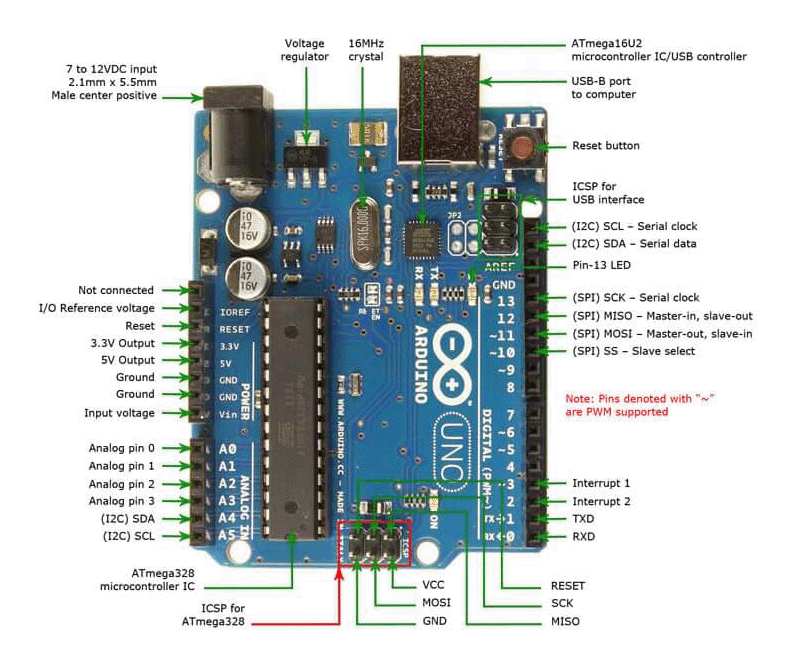
\includegraphics[width=0.65\textwidth]{imaxes/arduino-pinout.png}
	\caption{Connectivity diagram of Arduino UNO hardware development board}
	\label{fig:arduino}
\end{figure}

Arduino provides an IDE, which is a simplified integrated platform that helps users to develop software code efficiently using the C or C++ programming languages. The code written for the Arduino board is called a \textit{sketch}.

Arduino programming language is designed to be accessible and intuitive. It has several built-in functions.

There are two main functions that must be present in all sketches:

\begin{itemize}
	\item \texttt{void setup()}: first process run when Arduino starts. It runs once. Pin modes must be declared here.
	\item \texttt{void loop()}: this code will run endlessly.
\end{itemize}

Other commonly used predefined functions include:

\begin{itemize}
	\item \texttt{digitalWrite(pin, HIGH/LOW)}: sets the digital pin N state to HIGH (5V) or LOW (0V).
	\item \texttt{digitalRead(pin)}: : reads the value from a specified digital pin, either HIGH or
	LOW.
	\item \texttt{analogWrite(pin, value)}: writes an analog value to a pin.
	\item \texttt{analogRead(pin)}: reads the value of an analog pin.
\end{itemize}

There are predefined and third-party libraries that simplify the integration of specific
hardware and modules, such as NFC, WiFi and Bluetooth. These libraries
encapsulate advanced functionalities, reducing development complexity~\cite{Ref10}.

\subsection{ESP32}
\label{subsec:esp32}


The ESP32 is a low-cost, low-power microcontroller designed by Espressif Systems, mainly oriented to Internet of Things (IoT) applications. It is a versatile solution that combines Wi-Fi and Bluetooth connectivity in a single chip, allowing its integration in projects that require wireless communication, device control, and real-time data transmission~\cite{Ref11}.

One of the main features of ESP32 are:

\begin{itemize}
	\item \textbf{Processor:} Xtensa LX6 dual-core operating at
	frequencies up to 240 MHz.
	\item \textbf{Memory:} 520 KB of SRAM and support for up to 16 MB of external flash
	memory.
	\item \textbf{Connectivity:} Wi-Fi (802.11 b/g/n), Bluetooth 4.2 (BLE and BR/EDR).
	\item \textbf{Input/Output interfaces:}  Up to 32 multifunction GPIO pins, support for
	protocols such as UART, SPI, I2C, PWM, ADC (12 bits) and DAC (8 bits).
	\item \textbf{Compatibility with Libraries and Tools::}  Programmable using the ESP-IDF
	development framework or more accessible platforms such as Arduino IDE.
	Compatible with languages such as C/C++ and frameworks such as
	FreeRTOS for real-time applications.
\end{itemize}

\begin{figure}[h!]
	\centering
	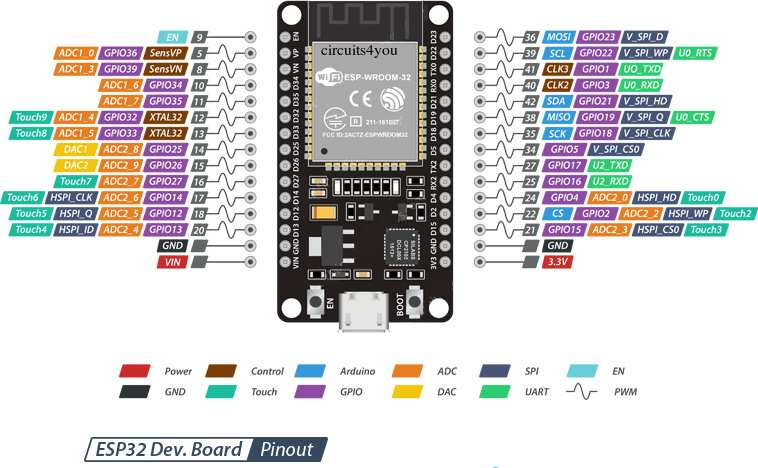
\includegraphics[width=0.8\textwidth]{imaxes/ESP32-Pinout.jpg}
	\caption{Connectivity diagram of ESP32 hardware development board}
	\label{fig:esp32}
\end{figure}






\subsection{Protoboard}
\label{subsec:protoboard}

For the design and testing of electronic circuits in the system, \textit{Protoboard}, also
known as breadboard, was chosen as the most appropriate tool for this purpose. It is
a rectangular plastic board containing an array of slots interrelated with thin plates of
copper, which though are internally connected within the board, also matting with
any electronic component without soldering it permanently. The central columns are
usually divided by a slot, separating two independent sections. Each column of five
holes is internally connected, facilitating the insertion of components and their
interconnection. To connect components together, their pins must be inserted into
the same column or cables must be used to connect different columns \cite{Ref14}.

The main purpose of a breadboard is to help easy and fast prototyping of the circuits,
so that the designer or students can assemble, reconfigure and test
different combinations quickly. The ability to create temporary connections on an
as-needed basis can be particularly helpful during the early stages of development,
where it is often necessary to make tweaks and optimizations to the design of a
given circuit. Also, its modular and reusable design renders it invaluable in both
academic and industrial settings.




\clearpage

\section{Cryptographic Mechanisms for NFC-Based Access Control}
\label{sec:crypto_mechs}
This section presents cryptographic mechanisms used to guarantee the confidentiality, integrity and authenticity of communications in access control systems.


\subsection{AES-128}
\label{subsec:aes128}

AES-128 is a symmetric encryption algorithm that uses a 128-bit key to protect data confidentiality and integrity. Its robust and efficient design makes it ideal for NFC-based access control systems.

During the AES-128 Encryption Process, a 128-bit block of data is taken along with a 128-bit key as input. The cipher goes through 10 rounds of transformations:

\begin{itemize}
	\item \textbf{Substitution (SubBytes):} Each byte is replaced by another byte using a substitution table (S-Box).
	\item \textbf{Shift (ShiftRows):} The bytes in the rows of the block are rearranged.
	\item \textbf{MixColumns:} The columns are combined to spread the data.
	\item \textbf{AddRoundKey:} Each round is combined with a key derived from the original.
\end{itemize}

Finally, the output is a 128-bit encrypted block of data. The receiver decrypts the data using the same key, ensuring that only authorized parties can access the information. The decryption process is the same as the encryption but reversing the order of the transformations~\cite{Ref12}.

\begin{figure}[H]
	\centering
	\includegraphics[width=0.7\textwidth]{imaxes/aes-128.png}
	\caption{AES-128 Encryption Process, including Substitution, Shift, MixColumns, and AddRoundKey}
	\label{fig:aes128}
\end{figure}


\subsection{HMAC-SHA256}
\label{subsec:hmac}

HMAC stands for \textit{Hash-based Message Authentication Code}. It is a cryptographic mechanism that ensures data integrity and authenticity by combining a cryptographic hash function with a shared secret key. Its purpose is to prevent unauthorized modification of transmitted messages and to verify the identity of the sender.

HMAC is meant to use a standard hash function, such as SHA-256, in combination with a secret key to generate an authentication code. If the key is longer than the block size of the hash function (64 bytes for SHA-256), it is truncated by applying the hash function; if it is shorter than 64 bytes, it is padded with zeroes.

An inner key is obtained by combining the key with a fill value called \texttt{ipad} (0x36 repeated). In addition, an outer key is obtained by combining the key with a fill value called \texttt{opad} (0x5C repeated).

The hash function is applied on the concatenation of the inner key and the message.  
Then, the algorithm is applied again on the concatenation of the outer key and the result obtained in the previous step. The whole equation applied is:

\[
\text{HMAC}(K,M) = H\big((K \oplus \text{opad}) \parallel H((K \oplus \text{ipad}) \parallel M)\big)
\]

where $K$ is the secret key, $M$ is the message, $H$ is the hash function, $\oplus$ represents the XOR operation, and $\parallel$ indicates concatenation~\cite{Ref21}.

MAC provides collision resistance, which takes advantage of the properties of the
underlying hash function, reducing the probability of two different messages
producing the same HMAC code. Also, it ensures protection against length extension
attacks, because the message is processed within a structure with a secret key
before the final application of the hash function, hash extension attacks are
mitigated.


\subsection{Hardware Security Module (HSM)}
\label{subsec:hsm}

A Hardware Security Module (HSM) is a dedicated, tamper-resistant piece of
hardware designed to generate, store and use cryptographic keys in a way that
keeps them isolated from potentially compromised general-purpose systems. In
essence, an HSM provides a “vault” for the most sensitive secrets (root keys,
certificate‐signing keys, master passwords, etc.) and enforces that any
cryptographic operation involving those keys happens entirely inside the module~\cite{Ref22}.

There are different types of HSM:

\paragraph{Physical HSM:}
\begin{itemize}
	\item Typically rack-mountable appliances that sit in a data-center.
	\item They connect to host systems over a secure network or PCIe interface and expose a well-defined API (such as PKCS\#11) for requesting cryptographic operations.
	\item Internally combine high-grade CPUs, hardware random-number generators, and physical tamper-sensors (which erase keys on attack).
\end{itemize}

\paragraph{Network-attached (or “cloud”) HSMs:}
\begin{itemize}
	\item Functionally very similar to physical HSMs, but located in a cloud provider’s data centers.
	\item Access is mediated via secure, often RESTful, APIs.
	\item Provide turnkey elasticity and geo-redundancy, but trust is required in the cloud vendor’s physical and personnel security.
\end{itemize}

\paragraph{Virtual HSMs (vHSMs):}
\begin{itemize}
	\item Software-only implementations that pretend to offer an HSM interface.
	\item Rely on software isolation (e.g., VMs or containers) rather than true hardware separation.
	\item Lighter weight and cheaper, but cannot guarantee the same level of protection against a compromised host.
\end{itemize}

\paragraph{Hybrid approaches:}
\begin{itemize}
	\item Embed a minimal “root” HSM in hardware or a vendor-provided trusted execution environment (e.g., TPM or ARM TrustZone), which in turn “unlocks” a software vHSM for day-to-day operations.
	\item Balances cost versus security: the hardware root protects the long-term keys, while the vHSM handles high-volume crypto.
\end{itemize}

\section{NFC}
\label{sec:nfc}

Near Field Communication (NFC) is a short-range wireless communication technology that enables data transfer between devices at a typical distance of 4 to 10 cm in non critical applications \cite{ref63} and $\geq 4$ cm in secure based applications \cite{ref64}. It is used in authentication and access control systems because of its security, ease of use and low power consumption. Thus, NFC systems are actually part of RFID technology, i.e. they can be considered as a subgroup within RFID techniques.

NFC uses an electromagnetic field to establish a connection between a reader device (active) and a tag device (passive). Data is transferred using secure protocols, following standards such as ISO/IEC 14443 \cite{Ref2}. Also, its limited range significantly reduces the risk of data interception.

NFC devices can operate in two modes:

\begin{itemize}
	\item \textbf{Reader/Writer:} The active device reads or writes data to the NFC tag.
	\item \textbf{Card Emulation:} An NFC device acts as a tag to be read by a reader.
\end{itemize}


\subsection{NFC UID}
\label{subsec:nfc_uid}

The UID (Unique Identifier) is a unique identifier assigned to each NFC tag, mainly used to uniquely identify each device in a system. This identifier can be static or dynamic, depending on the specifications of the NFC tag.

Static UID is the most common; it is immutable and serves as a unique identifier to validate access in simple systems. However, its ease of cloning represents a security risk in critical systems. On the other hand, dynamic UID is temporarily generated or variable at each interaction, it is usually encrypted and is much more secure than the static UID \cite{ref13}. It is used in advanced NFC cards and access systems that prioritize protection against attacks such as impersonation or cloning.


\subsection{MFRC522}
\label{subsec:mfrc522}

The MFRC522 module is an RFID/NFC reader/writer, which is based on NFC technology used for authentication and contactless payments at 13.56 MHz frequency. Its versatility and low cost made it a popular choice for many access control, electronic payment and inventory management applications. In addition, it supports ISO/IEC 14443A (MIFARE Classic, Ultralight and NTAG authentication). Its typical communication range is 1 to 3 cm, making it suitable for secure applications where physical proximity is required for authentication \cite{Ref15}.

Its low power consumption makes it ideal for embedded devices such as Arduino. Also, it includes a flexible communication interface compatible with different microcontrollers and communication protocols (SPI, I2C, UART). Security is provided through authentication with access keys in memory sectors, protecting the integrity of the data stored on the card. In addition its writing and reading capability allows the storage of information such as unique identifiers or balances in payment cards.


 \chapter{State of the Art}
\label{chap:state_of_the_art}

The objective of this section is to review current regulatory frameworks, hardware and software components, and advanced security schemes relevant to NFC-based access control.


\section{NFC Frameworks and Standards}

This section reviews the principal ISO/IEC standards that govern contactless cards interoperability, security and form factor. We examine ISO/IEC 14443 \cite{Ref23} for proximity communication protocols, ISO/IEC 7816-4 \cite{Ref24} for APDU-based command structures and ISO/IEC 7810 \cite{Ref25} for physical card dimensions.

\subsection{Contactless personal identification: ISO/IEC 14443}

ISO/IEC 14443 \cite{Ref23} is the international standard that defines how contactless identification devices (e.g., smart cards, RFID key fobs or NFC readers) should communicate at close range (up to about 10 cm) with reader stations.

It is structured in four complementary blocks that cover from the physical characteristics of the cards to the data exchange protocols and the mechanisms for managing multiple transponders simultaneously. An overview of each of these four components is presented below \cite{Ref65}:

\begin{itemize}
	\item \textbf{Part 1: Physical Characteristics.} Establishes the physical specifications of proximity cards, such as their size and format (ISO/IEC 7810 ID-1). It ensures that devices comply with a common physical standard, which is essential for hardware compatibility between different implementations.
	
	\item \textbf{Part 2: Signaling and transmission.} Defines the modulation and coding parameters of the signal. In Type A mode, ASK (Amplitude Shift Keying) modulation at 13.56 MHz with Manchester coding is used. In Type B mode, ASK-BPSK (Binary Phase Shift Keying) is used to avoid collisions. These schemes guarantee the robustness of wireless communication.
	
	\item \textbf{Part 3: Initialization and anti-collision.} Introduces the card detection and selection process. The anti-collision technique allows the identification of multiple cards within the reading field by assigning unique identifiers (UIDs). This feature is essential in environments where multiple cards may be present simultaneously.
	
	\item \textbf{Part 4: Transmission Protocol.} Details the exchange of commands and data between the card and the reader. It supports a transmission structure based on data blocks, where commands such as authentication, read, write and encryption are handled. This is critical in security applications, where a secure exchange of information is required.
\end{itemize}

Compliance with ISO/IEC 14443 ensures that both NFC chips and readers (e.g., NTAG424 DNA and PN532) operate under a standard and optimized protocol. The following aspects are key:

\begin{itemize}
	\item \textbf{Interoperability:} it allows the integration of different devices that follow the same standard, reducing compatibility issues between hardware and access control software \cite{Ref66}.
	
	\item \textbf{Security:} The standard supports authentication and encryption mechanisms at the protocol level, which is essential for protecting data in sensitive applications such as access control. In combination with algorithms such as AES-128 implemented in the NTAG424 DNA chips, the system can perform secure and encrypted authentication \cite{Ref67}.
	
	\item \textbf{Transmission efficiency:} The modular transmission structure ensures that data is exchanged quickly and reliably while maintaining low latency, which is crucial in real-time access systems.
\end{itemize}

\subsection{Identification cards communication: ISO/IEC 7816-4}

ISO/IEC 7816-4 \cite{Ref24} establishes the common language and the structure of the messages (APDUs) that allow a reader and a card to exchange instructions and data in an orderly and secure manner. This standard is key in applications that require authentication and secure transmission, such as NFC access control.

In this context, ISO/IEC 7816-4 specifies key technical aspects that enable these functionalities, including the use of APDU structures, system response management and transmission control protocols. These elements are described below to understand how they contribute to secure system operation \cite{Ref68}:

\begin{itemize}
	\item \textbf{APDU (Application Protocol Data Unit):} APDUs are the basis of communication between card and reader, divided into two types:
	\begin{itemize}
		\item \textit{Command APDU:} Contains the command, with a header consisting of the CLA (instruction class), INS (instruction), P1 and P2 (parameters) fields, together with the data and the Le (expected length of response) field.
		\item \textit{Response APDU:} Returns the requested data and the SW1 SW2 status code.
	\end{itemize}
	
	\item \textbf{Application Selection:} The SELECT command allows you to choose an application on the card based on its AID (Application Identifier), making it easy to interact with cards that manage multiple applications.
	
	\item \textbf{File Management:} The card manages structured data files, with READ, WRITE and UPDATE commands. These commands allow secure control of stored information.
	
	\item \textbf{Authentication and Encryption:} ISO/IEC 7816-4 supports authentication and encryption mechanisms through the use of keys, facilitating the implementation of AES or DES to secure communications.
\end{itemize}

In the NFC access control system, ISO/IEC 7816-4 enables secure transmission using APDUs, which support credential management and two-factor authentication. NTAG424 DNA chips, with AES-128 encryption capability, can be efficiently integrated using this standard to ensure that the exchanged data is protected and structured correctly.

\subsection{Contactless cards: ISO/IEC 7810}

ISO/IEC 7810 \cite{Ref25} defines the physical dimensions and general characteristics of identification cards, including NFC cards used in access control systems. This standard establishes specifications for the manufacture of ID cards in several standard formats, the most common being:

\begin{itemize}
	\item \textbf{ID-1 format:} 85.60 mm × 53.98 mm dimensions, typical of credit and debit cards.
	\item \textbf{ID-2 format:} 105 mm × 74 mm, like passport size.
	\item \textbf{ID-3 format:} 125 mm × 88 mm, used in passports and other travel documents.
	\item \textbf{ID-000 format:} 25 mm × 15 mm, smaller size format used in SIM cards.
\end{itemize}

Each format specifies a thickness of 0.76 mm \cite{Ref25}, providing consistency in the cards for handling and reading in devices. These standards enable interoperability in systems that require user identification and verification, ensuring that cards fit into readers and access control devices in a uniform manner.

ISO/IEC 7810 is especially relevant for identification and authentication applications, such as NFC-based access control systems. Standardized dimensions and physical properties ensure that cards remain uniform, which facilitates their integration into NFC devices and card readers. In addition, this standard allows the card design to be rugged and durable, withstanding repeated use in access control environments.



\section{NFC secure access control systems}

The following section reviews advanced NFC security schemes and their practical applications. In recent years, NFC technology has transcended its original use as a means of proximity reading to become the basis for multi-level security architectures. By combining cryptographic elements, challenge-response protocols and additional authentication factors, it is possible to ensure both data confidentiality and communication integrity. In addition, the integration of NFC with IoT platforms and cloud services enables dynamic and remote management of access to facilities \cite{Ref69}.

Before getting into advanced schemes, it is useful to understand the most common starting point for NFC access control applications: authentication by unique UID reading. This method simply consists of matching the unique identifier engraved on the chip with an authorized list on the server; its main virtue is simplicity, as it does not require complex cryptographic protocols or additional key exchange. However, since it is based exclusively on a static value that can be easily captured and duplicated, it lacks protection mechanisms against cloning or replay attacks.

These limitations are particularly evident when using cards such as MIFARE Classic, whose security has been widely compromised \cite{ref70} (see \ref{sec:NFCCards}). It is therefore necessary to contrast these ``basic'' systems with solutions that incorporate encryption, mutual authentication and other dynamic security factors.

\subsection{NFC Cards and PIN}

One robust security solution commonly offered related to the NFC technology is its combination with PIN authentication. Pins are short passwords, usually formed by numbers (although they may contain another type of characters), they are usually four to six characters long. On the one hand, PINS are easy to remember by humans. On the other hand, they are easy to guess or hack. In order to try to mitigate this, they usually have some kind of restriction regarding the number of tries an user has before being locked out \cite{ref30}.

The combination of these two technologies is based on the concept of multifactor authentication, users authenticate using something they have (NFC card) and something they know (PIN). There are two approaches in the usage of PIN in this type of system, using the same PIN for every user or using one for each user.

Leading companies like HID global offer several hardware solutions like the HID® multiCLASS SE® RK40 \cite{ref75}, figure~\ref{fig:hid_multiclass}, that is one single module including an NFC reader and a keypad.

\begin{figure}[h!]
	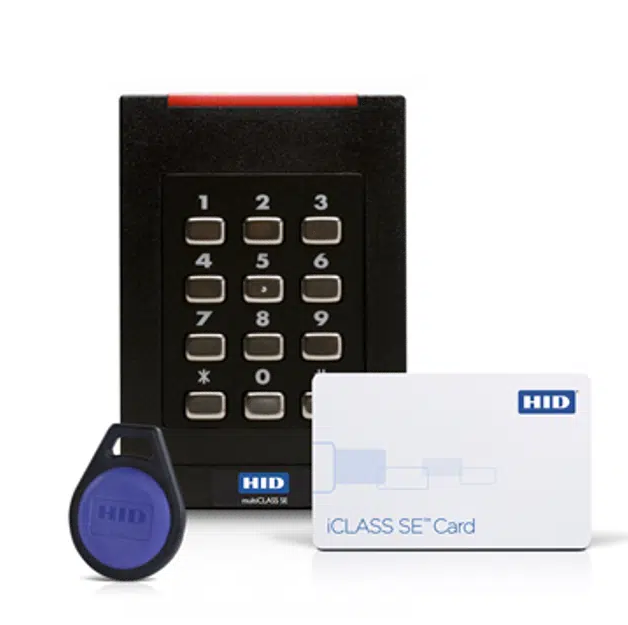
\includegraphics[width=0.6\textwidth]{imaxes/pinhid.png} 
	\caption{HID® multiCLASS SE® RK40 NFC PIN Reader, HID ICLASS SE card and tag}
	\label{fig:hid_multiclass}
\end{figure}

\subsection{NFC with Biometrics}

Biometrics are personal authenticators related to a physical human trait that can unequivocally identify a person. It should be permanent, measurable in a quick and easy way, and fast to compare against stored information.

The convergence of NFC technology with biometric authentication systems has given rise to advanced security and usability solutions in various fields. It is widely used in access control systems, secure payment methods and smartphone authentication \cite{ref83}. This integration allows the identification and verification of users in an efficient and secure manner, taking advantage of the benefits of both technologies. It is also based on the concept of multifactor authentication, where users authenticate using something they have (NFC card) and something they are (biometric).

Biometrics popularity is due to its lack of change during time, the most used biometric is the fingerprint, unique pattern of whorls and lines on the fingertips of a person. For centuries, it has been a reliable method of identifying people; from a crime record to a passport. Also, fingerprint readers use four different technologies: optical, which records an image; capacitance, ultrasonic and thermal, which identify and map ridges \cite{ref30}. There are also other biometrics that can be used but not to the same extent that are: hand geometry, iris, retina, face and voice.

\subsection{Enhanced Version 2 (EV2) NFC Mutual Authentication protocol}
\label{subsec:EV2}

Enhanced Version 2 (EV2) \cite{ref29} is NXP’s latest mutual-authentication scheme for NFC cards, built on ISO/IEC 14443-4 framing and AES-128 CMAC. EV2 ensures that both reader (PCD) and card (PICC) prove knowledge of a shared secret and derive fresh session keys on each transaction, protecting against replay, cloning and man-in-the-middle attacks.

Mutual authentication using AES-128 is a common practice in various industries that require secure communications and protection against unauthorized access. One of the most secure protocols in the access control industry which uses mutual authentication and AES-128 is SEOS \cite{ref31}, developed by HID and has its own SEOS cards. Which consists of an AES-128 encryption key for protecting data confidentiality and a MAC key that guarantees message integrity by means of authentication codes.

The EV2 exchange adheres to ISO/IEC 14443-4 command structure:
\begin{enumerate}
	\item The card is selected and detected, in which the reader is aware of the card and sends it a WAKE-UP command, which is responded with its corresponding ATQA (Answer to Request).
	\item The communication is established using the commands RATS (Request for Answer to Select) and ATS (Answer to Select).
	\item The reader sends an AES-128 encrypted challenge to the card. The card decrypts and responds with another encrypted challenge. If both challenges are successful, a secure channel is established.
	\item APDU (Application Protocol Data Units) commands are sent to read credentials inside the Seos™ Vault, the card returns the encrypted data, ensuring its integrity by means of the MAC key.
\end{enumerate}

In addition to SEOS, NXP’s broader MIFARE family, NTAG 424 DNA and DESFire EV2/EV3 \cite{ref32}, implements EV2 mutual authentication to different ends. NTAG 424 DNA’s EV2 protocol is trusted by vendors like RFID.it, Shenzhen Focused Smartech Co., Seritag, and ZipNFC \cite{ref84}; it follows the EV2 flow described above and activates CMAC-based confidentiality and integrity once the challenge–response succeeds (Figure~\ref{fig:ntag424_ev2}). MIFARE DESFire EV2/EV3 offers a comparable process but introduces variations in session-key handling and secure-messaging (IV + SM) to meet diverse application requirements.

\begin{figure}[h!]
	\centering
	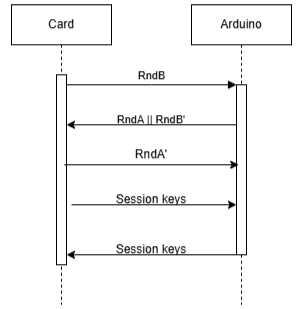
\includegraphics[width=0.7\textwidth]{imaxes/MA_diagram.png} % Cambia el nombre por tu imagen real
	\caption{NTAG424 mutual authentication diagram, random nonces and session keys exchange}
	\label{fig:ntag424_ev2}
\end{figure}

\subsection{NFC with Internet Of Things}

The Internet of Things (IoT) refers to a network of interconnected physical devices like sensors, actuators and embedded systems that communicate and exchange data over the Internet to enable intelligent automation and monitoring. The use of NFC, combined with the IoT, has enabled the development of advanced access control and management systems. These systems offer enhanced security, real-time traceability and greater automation compared to traditional methods based on static credentials. The combination of these technologies takes advantage of leverage short-range wireless communication capabilities to improve connectivity, interaction and management of IoT devices \cite{ref33}.

These systems are capable of implementing authentication and access control in secure infrastructures, managing assets in real-time, remotely monitoring through cloud platforms and automating processes without human intervention \cite{ref34}.

The most typical architecture of these types of systems is based on ESP32, which allows communication via the internet. Also, several devices can be part of these systems with different functionalities, the most remarkable in the access control field are:
\begin{itemize}
	\item Cameras: they use ESP32 to communicate
	\item Locks: they use ESP32 to communicate
	\item Smart Sensors: Devices that monitor environmental variables such as movement, and can communicate via NFC to turn on the lights.
\end{itemize}

There are several companies implementing these technologies such as Bosch Security and Safety Systems, which offer advanced access control solutions that integrate NFC and IoT technology. Its systems enable centralized access management in real time, using NFC-enabled mobile devices to authenticate users and control entrances to facilities. It is also interesting to mention Honeywell International, that has developed access control systems that incorporate NFC and IoT to provide secure authentication and efficient access management in corporate and industrial environments.

\subsection{NFC with Cloud}

Cloud services are remote computing resources such as storage, processing power and software applications hosted on distributed servers and accessed over the Internet. The combination of NFC and cloud services has boosted the development of advanced solutions for access management, authentication and user traceability. These systems allow data to be stored and processed on cloud servers, eliminating dependence on local storage and facilitating real-time access from any device with an Internet connection. In addition, they offer scalability, redundancy and advanced security through data encryption and multi-layered authentication \cite{ref35}.

There are some projects which can be used as examples of the different ways of implementing this technology. A cloud-based attendance management system that uses NFC cards to record employee check-in and check-out, reducing human error and increasing operational efficiency \cite{ref36}. These systems usually use TLS to communicate with the webserver, in this case, it sends the information with the UID of the NFC tag and records the hour the employee attended to the facilities in the webserver. Also, there are other projects that are similar \cite{ref37} that use the same function but in this case it uses the arduino database and a web server programmed in php which stores name, date and id. These resources can be hosted on AWS, Google Cloud or Microsoft Azure, which offer a higher level of scalability and security.

\subsection{NFC with Locks}

In the field of access control systems, there are various electronic lock technologies that differ according to their operating mechanisms, installation requirements and operating and maintenance costs. High-security mechanical locks, based on cylinders and latches reinforced with high-strength alloys, offer great robustness against physical attacks but are incompatible with centralized credential management solutions and have high maintenance costs. Electromechanical locks—such as electric frame locks or recessed solenoids—allow integration with card or code control systems by introducing a motorized actuator but have high power consumption and reduce their effectiveness after a certain number of mechanical cycles \cite{ref38}.

Stand-alone electronic locks, or ``smart locks'', incorporate microcontrollers, RFID or Bluetooth readers and internal batteries, which facilitate access management via smartphones, wireless networks or digital credentials, at the cost of a higher unit cost and a complexity of configuration and security that, if not properly managed, can introduce new vulnerabilities. Compared to these alternatives, magnetic locks stand out for their simplicity of construction, their durability and their ability to be integrated into large-scale infrastructures. These devices consist of an electromagnet rigidly fixed to the door frame and a ferromagnetic plate installed in the door leaf; when tension is applied, a holding force is generated that can exceed 600 kg, guaranteeing resistance to forced opening attempts.

With no moving parts, magnetic locks minimize mechanical wear and maintenance costs, and by operating in ``fail-safe'' mode, releasing the door when the power fails, they naturally meet evacuation requirements in emergency situations requiring immediate release of exits. In addition, their installation requires only two conductors and one signal contact, which simplifies wiring standardization and favors their adoption at multiple control points (gates, turnstiles, barriers), maintaining operational consistency and facilitating centralized management \cite{ref39}. Also, these types of locks allow the usage of REX (request-to-exit) devices, which release the door control mechanisms and facilitate safe egress.

\subsubsection{REX (request-to-exit)}

A Request-to-Exit (REX) sensor is an access control device that guarantees the free opening of an exit door fitted with an electric magnetic lock, without the need to enter credentials, by detecting the proximity of a person using infrared, microwave or laser scanning technologies; when activated, it sends a signal to deactivate the electromagnet and allow immediate passage. Equivalently, many installations use push buttons or panic bars mounted on the door leaf: their simple mechanical actuation interrupts the power supply to the maglock, releasing it instantly and ensuring both rapid evacuation and compliance with safety and accessibility regulations. Solutions such as ASSA ABLOY's Aperio systems \cite{ref40} or Bosch Security Systems' security doors \cite{ref41} often integrate REX sensors and push-button or panic bar optics interchangeably, adapting to the operational and compliance needs of each environment.


\section{NFC cards}
\label{sec:NFCCards}

This section presents the main families of NFC cards used in identification and access control applications, with special emphasis on their technical characteristics, storage capacities and security mechanisms. Although there are multiple manufacturers of NFC-compatible chips and cards, the market for secure identification solutions is largely dominated by NXP Semiconductors \cite{ref80}. It develops the most widely used NFC cards, including MIFARE, DESFire, NTAG and SmartMX. Also, there are other companies such as Infineon Technologies, which offer secure NFC tags too, such as the OPTIGA Authenticate and secure memory chips \cite{ref82}. In this section, MIFARE Classic is exposed due to its importance in the early stages of this technology, which then leads to the evolution into other cards that support cryptographic operation for increased security, such as NTAG424.

\subsection{MIFARE Classic and similar NFC cards}

MIFARE Classic \cite{Ref28}, figure~\ref{fig:mifare_classic} \cite{ref81}, is a model of NFC card that was introduced as a cost-effective and widely compatible solution, operating in the 13.56 MHz band and based on the ISO/IEC 14443-A standard. These cards offer limited storage capacity, designed primarily for simple applications such as public transportation, basic access and small payments. They were pioneers in identification systems, enabling popularization of the use of NFC. Also, due to their low cost and simplicity, they were massively implemented in environments with basic security needs.

MIFARE Classic are vulnerable to cloning attacks due to their Crypto1 encryption scheme, considered weak by current standards \cite{ref70}. These vulnerabilities have limited their use in applications requiring high levels of security. The model of cards is gradually being replaced by more secure technologies such as MIFARE DESFire or NTAG 413 DNA, which implement advanced encryption such as AES \cite{ref71}. However, widespread deployment and cost constraints mean that many organizations still rely on these insecure cards, delaying a full migration to more robust alternatives.

\begin{figure}[h!]
	\centering
	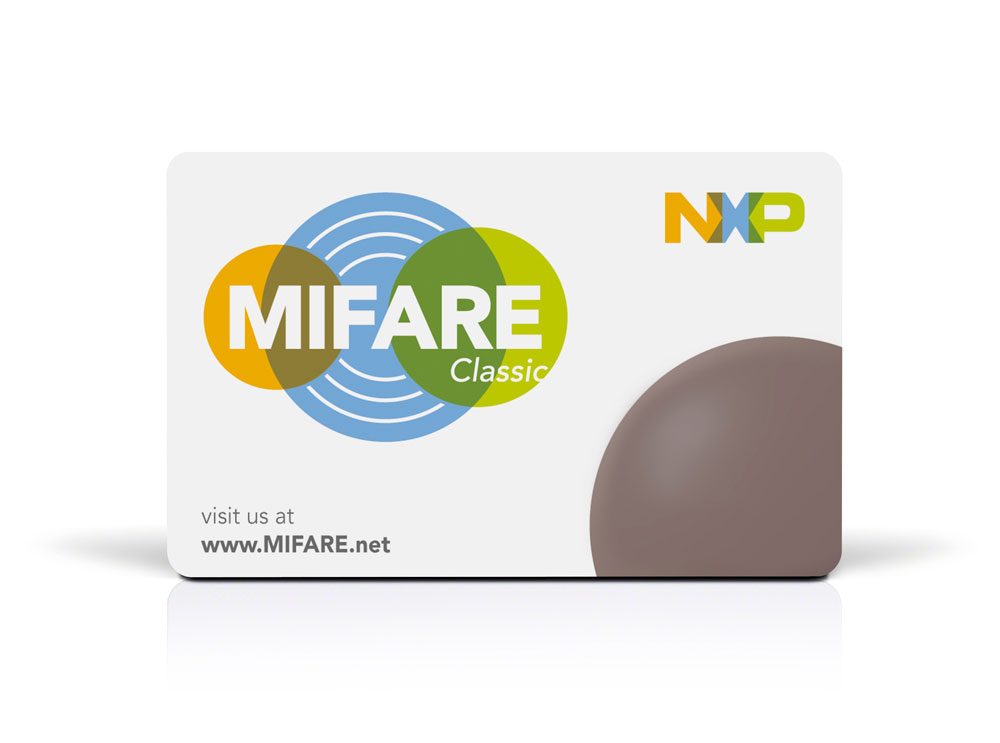
\includegraphics[width=0.4\textwidth]{imaxes/mifare1.jpg} % Cambia el nombre por tu imagen real
	\caption{MIFARE Classic card}
	\label{fig:mifare_classic}
\end{figure}

\subsection{NTAG 424 DNA}

With the growing demand for security, new solutions in the NFC card field have emerged, such as the NTAG 424 DNA \cite{ref29} cards, developed by NXP Semiconductors, which offer significant improvements over their predecessors. This card incorporates the AES-128 encryption standard, providing stronger protection against cloning attempts and unauthorized access. Also, they integrate SUN (Secure Unique NFC) Authentication technology, which allows the generation of unique and secure messages in each interaction, ensuring the authenticity of the communication and preventing replay attacks. Importantly, NTAG 424 DNA fully supports the Enhanced Version 2 (EV2) mutual-authentication protocol, allowing them to establish secure channels with NFC readers.

NTAG 424 DNA is able to generate unique and random identifiers for each transaction, enhancing user privacy and preventing unauthorized tracking. In addition, they are designed to be fully compatible with standard NFC devices, facilitating their integration into mobile applications and modern systems. Last but not least, one of the key features of this card is its communication speed, which can be highlighted in faster data transfer rates and improving efficiency in operations that require real-time information exchange.

\subsection{Key Management with NTAG424}
\label{subsec:keymanagement}

The NTAG 424 DNA card integrates a robust cryptographic key management system designed to ensure secure and flexible access control and data protection. This system is based on key hierarchy and diversification, allowing for the generation of unique keys per tag and application, while maintaining compatibility with shared functionalities when necessary.

As described in Section 8.2.4 of the official NXP datasheet \cite{ref42}, the card supports a key diversification mechanism using a Master Personalization Key (or Master Secret) that is securely stored and managed in the backend infrastructure. This master key is used only during initialization or key regeneration processes to derive diversified keys.

The NTAG 424 DNA supports five distinct 128-bit AES keys, each with specific roles in the authentication and access control structure:

\begin{itemize}
	\item \textbf{AppKey0}: Used for mutual authentication Enhanced version 2 (EV2) standard, as seen in figure~\ref{fig:ntag424_ev2} \cite{ref42}, and read access to NDEF (NFC Data Exchange Format) files.
	\item \textbf{AppKey1}: Enables writing to NDEF files and allows verification of data integrity via CMACs.
	\item \textbf{AppKey2}: Grants access to proprietary data files that may contain sensitive or application-specific information.
	\item \textbf{AppKey3}: Controls access to advanced security features, such as SDM (Secure Dynamic Messaging), which allows protected reading of encrypted and integrity-checked data.
	\item \textbf{AppKey4}: Reserved for extended functionalities and future implementations.
\end{itemize}

Each key slot supports a Key Version Byte (1 byte) that identifies the current version of the key, enabling efficient management and update of credentials. This feature is particularly useful in systems where key rotation or renewal is a security requirement. Moreover, the tag allows for key updating and configuration through authenticated sessions using the ChangeKey and ChangeKeySettings commands. These operations can only be performed after a successful mutual authentication, ensuring that key management remains secure and protected against unauthorized access.

This architecture provides a balance between security, scalability, and flexibility, making the NTAG 424 DNA suitable for a wide range of secure NFC applications, including access control, secure identification, and ticketing systems.

\begin{figure}[h!]
	\centering
	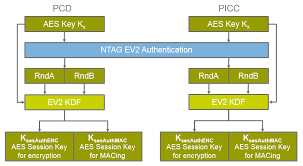
\includegraphics[width=0.8\textwidth]{imaxes/EV2ntag.png} % Cambia el nombre por tu imagen real
	\caption{NTAG EV2 Authentication using AES-128 encryption: on the left PCD (reader) and on the right PICC (NTAG)}
	\label{fig:ntag424_ev2}
\end{figure}

\section{Libraries and modules for NFC readers}

In the Arduino ecosystem and compatible microcontrollers, two of the most commonly used reader-library combinations for working with NTAG424 DNA cards are the following.

\subsection{MFRC522\_NTAG424DNA}

The MFRC522\_NTAG424DNA library \cite{ref26} facilitates the interaction of a microcontroller (e.g., Arduino) with NFC NTAG424 DNA cards through the MFRC522 reader. It aims to provide a simple and robust interface for identification, data read/write and key management operations in secure applications (access control, traceability, etc.).

The NTAG424 DNA supports three communication modes, differentiated by the level of protection and the integration of cryptography. Each functionality has three associated functions depending on the level of security needed:

\begin{itemize}
	\item \textbf{Plain Mode:} Plain text communication (without cryptography) and allows basic read/write operations and UID reading without prior authentication. It is useful for testing or low security scenarios.
	
	\item \textbf{MAC Mode:} In this mode each command is accompanied by a ``Message Authentication Code'' (MAC) calculated with AES-128, guaranteeing the integrity and authenticity of the commands and preventing alterations in transit. It requires the user to provide the AES key (16 bytes) and the key number (\texttt{keyNumber}).
	
	\item \textbf{Fully Secure Mode:} It establishes an end-to-end encrypted channel after AES-128 mutual authentication. All exchanged data (commands and responses) travel encrypted, protecting confidentiality, making it ideal for high security applications: critical access control, contactless payment, etc.
\end{itemize}

For reading the UID, there are two different functions depending if we are using random or fixed UIDs:

\begin{itemize}
	\item \texttt{DNA\_StatusCode DNA\_Full\_GetCardUID(byte* backUID\_7B)}: this function is used to read fixed UIDs.
	\item \texttt{void DNA\_Plain\_GetCardUID(byte* backUID\_7B)}: this function is used to read random UIDs.
\end{itemize}

For reading data, there are two different functions depending if the user needs to read a file or a whole memory page:

\begin{itemize}
	\item \texttt{ntag424\_ReadData(uint8\_t file, uint8\_t offset, uint8\_t *buffer, uint8\_t length)}: Allows data to be read from a specific file on the NTAG424 card. Parameters allow the user to specify the file that is being read, the offset which indicates the initial position where the data will start to be read, the buffer where the read data will be stored and the length in bytes of the data.
	
	\item \texttt{ntag424\_ReadPage(uint8\_t page, uint8\_t *buffer)}: It is an auxiliary function that allows the user to read a whole page in the case that memory is divided into fixed pages.
\end{itemize}

As well as reading a card, the writing process depends if the user wants to write a file or a memory page:

\begin{itemize}
	\item \texttt{ntag424\_WriteData(uint8\_t file, uint8\_t offset, uint8\_t *data, uint8\_t length)}: The parameters are analogous to the corresponding reading function.
	\item \texttt{ntag424\_WritePage(uint8\_t page, uint8\_t *data)}: Writes directly a page of memory.
\end{itemize}

Last but not least, this library includes some functions to cover the functionalities of authentication and key management:

\begin{itemize}
	\item \texttt{ntag424\_AuthenticateAES(uint8\_t keyNumber, uint8\_t *key)}: Performs mutual authentication using an AES-128 key. It allows the user to select which of the keys will be used to establish a secure session.
	
	\item \texttt{ntag424\_ChangeKey(uint8\_t keyNumber, uint8\_t *newKey)}: Once mutual authentication has been successfully established, this function allows updating the AES key associated with the specified \texttt{keyNumber}, replacing the old key with a new (16-byte) key.
\end{itemize}

Also, this library implements a system with several status codes, documented in the README of the GitHub, which help the developer to document the different errors that could appear during the course of the project. The code ``0'' represents a successful operation and the codes ``1--34'' the different errors that can be found. Finally, regarding the integration with the Arduino IDE, this library is included in the library manager, which means that the user can install it directly from it and all the dependencies will be managed automatically by the IDE.

\subsection{Adafruit-PN532-NTAG424}

The Adafruit-PN532-NTAG424 library \cite{ref27} is another tool for interfacing with the NTAG424 DNA chips and the PN532 reader, both essential elements in the development of secure access control systems based on NFC technology. This repository allows developers to integrate advanced security functionalities into their projects, focused on access protection through authentication and encryption.

This library provides a set of functionalities that enable robust interaction between the microcontroller and the NTAG424 DNA chips. These NFC tags are highly secure due to their ability to handle AES-128 encryption and SUN (Secure Unique NFC) signatures. The main features of this library include:

\begin{itemize}
	\item \textbf{Support for NTAG424 DNA:} The use of NTAG424 DNA chips ensures an advanced level of security in authentication applications, which is essential in access control systems. The library allows reading and writing data in these tags, in addition to performing cryptographic operations such as authentication and SUN signature generation.
	
	\item \textbf{AES-128 encryption:} As in other advanced libraries, Adafruit-PN532-NTAG424 supports AES-128 encryption, which ensures that the data transmitted between the tag and the reader is secure. This helps prevent cloning or spoofing attacks.
	
	\item \textbf{PN532 reader compatibility:} The library is designed to work natively with the PN532 reader, one of the most popular readers in the NFC developer community. This ensures that the hardware used in the project can be easily integrated and managed with this tool.
\end{itemize}


\section{Integrated circuit communication protocols}

This section presents the linking mechanisms used for the interconnection between the different modules of the embedded system, and discusses each protocol in terms of its operation, advantages and disadvantages in the context of an NFC-based access control system.

\subsection{Serial Peripheral Interface (SPI)}

SPI (Serial Peripheral Interface) \cite{ref17} is a synchronous communication protocol developed by Motorola in 1979 to allow serial data transmission between microcontrollers and peripheral devices such as sensors, EEPROM memories, A/D converters and communication modules. Its design is based on four main signal lines:

\begin{itemize}
	\item \textbf{SCLK (Serial Clock):} Clock signal generated by the master to synchronize communication.
	\item \textbf{MOSI (Master Out - Slave In):} Data line used to send information from the master to the slaves.
	\item \textbf{MISO (Master In - Slave Out):} Data line used to transmit information from the slave to the master.
	\item \textbf{SS (Slave Select):} Selection line that allows the master to activate or deactivate communication with a particular slave.
\end{itemize}

SPI operates on a single-master scheme, where a single master device controls the communication and selects the slaves via SS control signals. Unlike other protocols such as I2C, it does not require device addresses, which allows for faster and more efficient data transfer, albeit with more physical connections \cite{ref16}.

SPI defines four modes of operation based on two parameters:

\begin{itemize}
	\item \textbf{CPOL (Clock Polarity):} defines the inactive state of the clock (high or low).
	\item \textbf{CPHA (Clock Phase):} Determines on which clock edge (rising or falling) the data is transmitted and sampled.
\end{itemize}

\begin{table}[H]
	\centering
	\begin{tabular}{|c|c|c|l|}
		\hline
		\textbf{Mode} & \textbf{CPOL} & \textbf{CPHA} & \textbf{Description} \\ \hline
		0             & 0             & 0             & Data captured on rising edge and sent on falling edge. \\ \hline
		1             & 0             & 1             & Data captured on falling edge and sent on rising edge. \\ \hline
		2             & 1             & 0             & Data captured on falling edge and sent on rising edge. \\ \hline
		3             & 1             & 1             & Data captured on rising edge and sent on falling edge. \\ \hline
	\end{tabular}
	\caption{SPI modes of operation}
	\label{tab:spi_modes}
\end{table}

There are some advantages that SPI offers in relation to other protocols. It provides high-speed communication without a defined maximum transfer rate. Also, it can transmit and receive data simultaneously (Full-duplex). Furthermore, one of its more outstanding features is its low consumption of computational resources, since it does not require additional processing for error control or addressing.

However, SPI has some limitations as well. It requires more physical lines compared to protocols such as I2C, which can be a problem in systems with multiple devices. Moreover, it does not include data reception confirmation mechanisms (ACK/NACK); neither does it support multi-master communication.

\subsection{UART (Universal Asynchronous Receiver-Transmitter)}

The UART (Universal Asynchronous Receiver-Transmitter) protocol is one of the most widely used methods for transmitting data between electronic devices. It is an asynchronous serial communication protocol that allows the communication between microcontrollers, computers and other embedded devices without the need for a shared clock signal.

UART is a communication protocol based on sending serial data, which means that it transmits bits one by one over a data line. Unlike other protocols such as SPI or I2C, when UART is being used, each device manages its own internal timing based on a predefined baud rate.

UART data packets include the following elements:

\begin{itemize}
	\item \textbf{Start Bit:} Indicates the start of transmission by lowering the data line from a high state to a low state.
	\item \textbf{Data bits:} These can be from 5 to 9 bits, depending on the configuration. Normally, they are sent in order of lowest to highest weight.
	\item \textbf{Parity Bit (Optional):} Used for error detection by checking whether the number of bits in '1' is odd or even.
	\item \textbf{Stop Bits:} Indicate the end of transmission by taking the data line to a high state for one or two cycles \cite{ref18}.
\end{itemize}

For UART communication to be successful, both devices must be configured with the same parameters:

\begin{itemize}
	\item \textbf{Baud Rate:} Data transmission rate in bits per second (bps).
	\item \textbf{Number of Data Bits:} Generally 8 bits in modern systems.
	\item \textbf{Parity:} Can be none, even or odd, depending on whether error checking is required.
	\item \textbf{Stop Bits:} Usually 1 or 2 bits.
\end{itemize}

 \chapter{Planning and Methodology}

Before getting into details on the system design and development, this section will explain the selection of the engineering methodology and the way it is applied in this project.

\section{Methodology}

A Kanban board is used to manage project tasks using an incremental method, organizing them into \textit{To Do}, \textit{In Progress} (further divided into \textit{Working} and \textit{Waiting}) and \textit{Done} columns. This structure avoids bottlenecks and facilitates visibility of the status of each activity. Moreover, by focusing on reducing waste (overproduction, unnecessary movements, defects, overprocessing and waiting), it minimizes downtime and optimizes workflow \cite{ref43}. In addition, an initial project planning will be performed, progress will be monitored, deviations will be adjusted and regular meetings will be held with the director.

Also, prototyping is used for the assembly and functionality development of hardware modules. It helps to rapidly develop and test new ideas and designs before final production. In hardware design, prototyping is essential to validate concepts, explore design alternatives and detect problems early on. It is an iterative process in which multiple versions of the design are created, tested and refined; allowing adjustments and improvements based on continuous testing and feedback \cite{ref44}. In this project, every module that is intended to be added to the project is tested in an isolated way, before adding it to the complete system, to check whether it is able to perform all its functionalities.

\subsection{Hardware Prototyping Planning}

The adoption of an iterative development cycle at the hardware layer is intended to validate physical components (Arduino Uno, MFRC522 and ESP32) independently, allowing for quick adjustments to wiring, SPI/UART configurations and test codes before advancing to the next phase.

In order to adopt this methodology, the following iterations were defined:

\begin{itemize}
	\item Iteration 1: Basic NFC communication.
	\item Iteration 2: Providing basic Wi-Fi connectivity.
	\item Iteration 3: Mutual authentication and writing in NFC card Memory.
	\item Iteration 4: Reading NFC Card memory and Loading Cryptographic Keys.
	\item Iteration 5: NACU Subsystem Full Integration.
	\item Iteration 6: Magnetic lock Management for Physical Access Control.
\end{itemize}

\subsection{Incremental Planning for Backend \& HSM}

To adapt incremental development to the Django server and HSM logic, five delivery cycles were defined with several deliverables attached to each one of them:

\begin{itemize}
	\item Iteration 1: Basic Structure and Authentication.
	\item Iteration 2: Key Derivation System.
	\item Iteration 3: Transport encryption (HTTPS/TLS).
	\item Iteration 4: Real Time Access Control Mail Alert System.
	\item Iteration 5: Role-Based Access Control.
\end{itemize}

\subsection{Deliverables}

\begin{table}[H]
	\small
	\begin{tabular}{|c|p{5cm}|c|p{3.5cm}|}
		\hline
		\textbf{Code} & \textbf{Description} & \textbf{Iteration} & \textbf{Validation} \\ \hline
		1  & Setup Django project with login and admin default panel. & 1 & \multirow{4}{*}{\parbox{3.5cm}{Persistence of UIDs and verification of time slots.}} \\ \cline{1-3}
		2  & Persistence of UIDs and verification of time slots. & 1 & \\ \cline{1-3}
		3  & Create a view that allows visualization of access attempts. & 1 & \\ \cline{1-3}
		4  & Create data models for users and schedules. & 1 & \\ \hline
		5  & Create endpoints for submitting and authenticating users. & 1 & \multirow{3}{*}{\parbox{3.5cm}{JSON response with 32 hex key characters.}} \\ \cline{1-3}
		6  & Endpoint for HMAC-SHA256 key derivation. JSON response with 32 hex key characters. & 2 & \\ \cline{1-3}
		7  & Software implementation of Hardware Security Module. & 2 & \\ \hline
		8  & File I/O management and error control. & 2 & \multirow{2}{*}{\parbox{3.5cm}{Secure connection https:// encrypted in development.}} \\ \cline{1-3}
		9  & Evolution to HTTPS. Secure connection https:// encrypted in development. & 3 & \\ \hline
		10 & Wi-Fi module adaptation for working with HTTPS. & 3 & \multirow{2}{*}{\parbox{3.5cm}{Receiving emails after unauthorized access.}} \\ \cline{1-3}
		11 & SMTP configuration. Receiving emails after unauthorized access. & 4 & \\ \hline
		12 & Code functionality to send mail. & 4 & \multirow{2}{*}{\parbox{3.5cm}{Prototype.}} \\ \cline{1-3}
		13 & Reader detection. Prototype. & 5 & \\ \hline
		14 & Creation of Role model. & 5 & \\ \hline
	\end{tabular}
	\caption{Incremental Methodology list of Deliverables for the different iterations of the incremental ACMS development}
	\label{tab:deliverables}
\end{table}


\section{Project Planning, Monitoring and Controlling}

This section describes the processes and tools used to ensure that prototype development met its objectives in terms of scope, schedule and budget. Emphasis is placed on continuous planning, monitoring and control of tasks to ensure on-time delivery, traceability of changes and compliance with quality criteria throughout the project life cycle.

\subsection{Monitoring Tools}

\paragraph{Kanban:} For both iterative and incremental prototyping development, a Kanban board was used with \textit{To Do}, \textit{In Progress}, \textit{Test} and \textit{Done} columns. Each board describes a specific task (e.g: UID read, EV2 authentication, NDEF write, endpoint creation).

\begin{figure}[H]
	\centering
	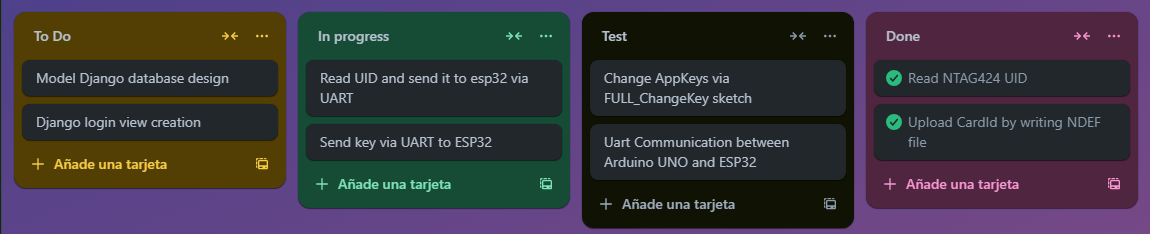
\includegraphics[width=0.7\textwidth]{imaxes/kanban.png} % Insert your image path here
	\caption{Kanban Board at Early Stages of the Project}
	\label{fig:kanban}
\end{figure}

\paragraph{Version control on GitHub:} During the development of both the Arduino/ESP32 scripts and the Django/HSM backend, each progress is recorded through “commits” in a single repository on GitHub. In this way, a detailed history of changes to all project components is maintained, facilitating collaboration, version tracking and retrieval of previous states when necessary \cite{ref52, ref53}.

\subsection{Gantt Chart and Timing Resources}

A Gantt chart was developed in Excel to estimate the “goals” of each iteration and their approximate duration (total 300 hours).

Main phases:
\begin{itemize}
	\item State of the Art research.
	\item Write project draft.
	\item Researching on Arduino Uno, MFRC522 and ESP32 technology.
	\item Researching on NTAG424 technology.
	\item System design and analysis.
	\item Iterative hardware prototyping.
	\item Testing MFRC522-NTAG424 functionalities.
	\item Incremental backend Access Control Management Server implementation.
	\item Full system integration and testing.
	\item Degree thesis.
\end{itemize}


\begin{figure}[H]
	\centering
	\includegraphics[width=20cm]{imaxes/gantt1.png} % Insert your image path here
	\caption{Gantt Diagram representing all the phases of the project and the time in weeks that was spent on each one, along with its deviation from the original duration}
	\label{fig:gantt}
\end{figure}

\subsection{E2E Validation and Testing}

After each hardware iteration, manual tests (NFC read/write) were executed.

On the hardware, simple tests were performed on each iteration to ensure proper communication worked.

On the backend, functional tests were performed using petitions in the browser to REST endpoints and mail tests (SMTP).

Finally, several tests were performed on the final system to ensure its capacity to consequently perform the tasks necessary for the data flow to function.

\subsection{Materials and Cost Estimate}

This section details the material resources and their associated cost for the development, deployment and testing of the prototype. All prices are approximate, obtained from online stores as of this writing.

\paragraph{Prototyping and access control hardware:}

\begin{itemize}
	\item Arduino Uno: 22 €.
	\item MFRC522 module (NFC reader): 8 €.
	\item ESP32 module: 10 €.
	\item Standard protoboard (830 points): 5 €.
	\item Basic wiring (male-male jumpers, USB, power supply): 6 €.
	\item Dollatek DC 0-5 V relay module: 7 €.
	\item Electric magnetic lock LIBO 12 V, 180 kg: 28.59 €.
	\item Power adapter 12 V 1.5 A: 8 €.
	\item DC 12 V male-female adapter: 4 €.
\end{itemize}

Total access control hardware: 98.59 €.

\paragraph{Development and testing infrastructure:}

\begin{itemize}
	\item Personal Computer (Django server development and testing): Cost valued at 1,200 € with estimated useful life of 4 years → 0.82 €/day.
	\item Browsers for testing (Opera and Microsoft Edge): no additional cost (free software).
	\item Total software and PC infrastructure (180 days estimated): 147.60 €.
\end{itemize}

\paragraph{Human resources:}

For this project, the working personnel are:

\begin{itemize}
	\item A responsible for system design and implementation, whose cost was estimated using the calculator provided by the UDC \cite{ref60}, which resulted in a total cost of 28,574.31 €.
	\item A project manager role, represented by the tutor whose work was estimated to last 45 hours at a cost of 100 € per hour, resulting in 4,500 €.
\end{itemize}

Total human resources cost (320 hours estimated): 8,151.5 €.

\begin{table}[H]
	\centering
	\begin{tabular}{|l|r|}
		\hline
		\textbf{Resource} & \textbf{Cost} \\ \hline
		Hardware & 98.59 € \\ \hline
		Software & 147.60 € \\ \hline
		Human & 8,151.5 € \\ \hline
		\textbf{Total} & \textbf{8,397.69 €} \\ \hline
	\end{tabular}
	\caption{Hardware, Software and Human costs of the project}
	\label{tab:costs}
\end{table}

 \chapter{Development}

The objective of the development of the system is to create a modular, open source,
cost-effective access control system using NFC technology to securely manage
electronic locks and record entry events in real time. This section describes in a
comprehensive way how the access control system has been conceived and built in
two main blocks, the NFC Access Control Unit (NACU) and the Access Control
Management Server (ACMS),following a modular and open source approach that
facilitates the independent development of each component and its future expansion,
while keeping costs low thanks to inexpensive hardware.
In this chapter, the overall system architecture and the personal authentication data
flow is outlined, showing how key derivation and HMAC signing are handled by a
simulated HSM. Then, the iterative development of the NFC Access Control Unit
(NACU) and the step‑by‑step implementation of the Django‑based Access Control
Management Server (ACMS) are summarized. Finally, end‑to‑end validation tests
that demonstrate the system’s ability to securely control and log physical access are
presented.

\section{System Design}
\label{sec:SystemDesign}
The architecture design of the system is ment to provide secure and flexible physical
access control via NFC. It aims to ensure that only authorized users can open doors
or barriers, while centrally logging each access attempt. Also, it ensures consistency
in access policies, the possibility of implementing updates and new functionalities
without physically intervening on each device, and a high level of cryptographic
security to protect both credentials and communication between the two domains.
For this purpose, it is divided into two main modules as exposed in the Figure~\ref{fig:arch}:

\begin{itemize}
	\item \textbf{NFC Access Control Unit (NACU).}  Consisting of the NFC reader
	(MFRC522), the Arduino UNO microcontroller, the ESP32 Wi-Fi module and
	the magnetic lock.
	\item \textbf{Access Control Management Server (ACMS).}  Implemented on Django with SM and model database.
\end{itemize}

This architecture responds to the challenge of providing reliable and flexible access
control. The NACU acts as a “light terminal” \cite{ref62} that only reads raw credentials,
generates nonce and executes only opening commands. By delegating all
cryptographic logic and permission decisions to the server, we reduce the risk of key
leakage and simplify firmware in the field.
However, the ACMS centralizes the business logic, role management and
authorization schemes. By using a single point of truth for roles and schedules,
facilitates consistency and deployment of changes without physically visiting each
unit. Also, the HSM stores the MasterKey and performs all key derivation, ensuring
that even a server breach cannot directly expose live card keys.

\begin{figure}[H]
	\centering
	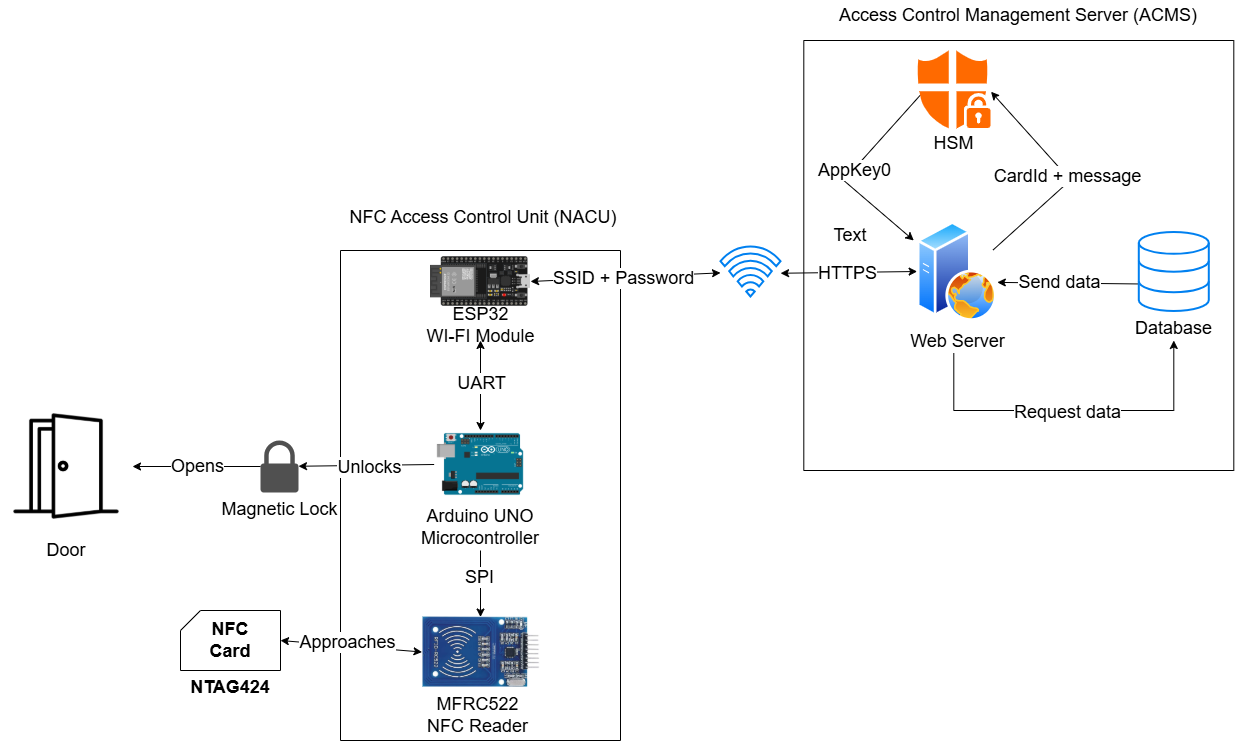
\includegraphics[width=\textwidth]{imaxes/Arqu.png}
	\caption{NFC Physical Access Control System Architecture. Left part of the figure represents the physical door with a
		magnetic lock, connected with the NACU module with an NFC Reader. The right part represents the ACMS server
		authentication module}
	\label{fig:arch}
\end{figure}

\subsection{Personal Authentication Data Flow}

When the users arrive at the physical facility and want to unlock the door to gain
access they tap their personal NFC card on the reader to identify themselves,
starting the personal authentication data flow. This Implementation employs the
ISO/IEC 14443‑4 EV2 mutual‑authentication protocol to verify the card’s authenticity
before proceeding with UID reading. 

Figure~\ref{fig:flow_auth}  describes the designed personal authentication protocol data flow, that summarizes the following operation:

\begin{enumerate}
	\item It starts as soon as the card approaches the NFC Access Control Unit
	(NACU).
	\item The reader, instead of first requesting an application key, reads directly the card identifier (CardId) stored in the NDEF file in Plain mode.
	\item The NACU sends to the Access Control Management Server (ACMS) a
	request including the CardId and a contextual message (“READUIDN”) that
	allows to differentiate the origin of the request.
	\item The server forwards this information to the HSM module, which computes an
	HMAC-SHA256 on the CardId and the message using the MasterKey and
	returns a 16 bytes AppKey0 to the ACMS, which forwards it to the NACU.
	\item With AppKey0 the protected reading procedure of the card UID is unlocked
	using the EV2 mutual authentication protocol, finally obtaining the UID.
	\item This UID is sent back to the ACMS, which compares it with its database of
	users and time slots to decide whether to authorize or deny access, returning
	the result to the NACU.
\end{enumerate}

\begin{figure}[H]
	\centering
	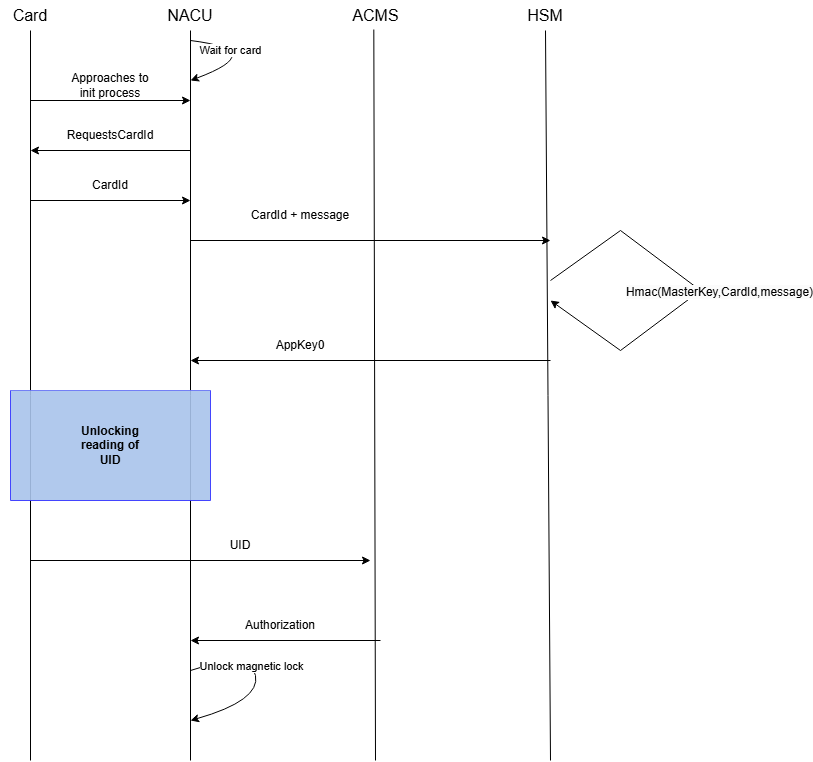
\includegraphics[width=\textwidth]{imaxes/DataFlow}
	\caption{General Personal Authentication Data Flow of the Final System, from the Approach of the card to the NACU, to the final Authorization}
	\label{fig:flow_auth}
\end{figure}

In Figure ~\ref{fig:nacu_states}  it is shown how each step of the data flow is managed as a different state as a loop in the microcontroller, so that the system proceeds in an orderly
fashion from card detection to final authorization, ensuring that each action is
executed only when appropriate within the defined flow. When a card is tapped, the
NACU sends its CardId to the ACMS and waits for the derived AppKey0. It then
receives AppKey0 and uses it to securely read the UID and send it to the ACMS.
Depending on the authorization ACMS response, the magnetic lock opens or
remains closed and the process ends. At each state in which a response from ACMS
is expected, a timeout ensures the reader resets and remains operational in case of
communication failure.

\begin{figure}[H]
	\centering
	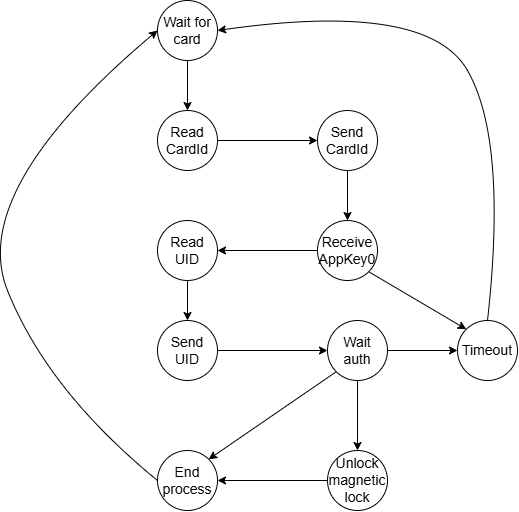
\includegraphics[width=\textwidth]{imaxes/stateD}
	\caption{ NACU state diagram for personal authentication using NFC cards}
	\label{fig:nacu_states}
\end{figure}

\subsection{Key Management System}

The system developed in this project employs a hierarchical and diversified key
management scheme (Figure~\ref{fig:key_management}), according to the strategy recommended by NXP
for the NTAG424 DNA \cite{ref42}. Each NTAG424 DNA card has a unique MasterKey,
which does not leave the trusted environment and is used only to derive four
application keys (AppKey0-AppKey3) that enable the different functionalities
available in FULL mode (\ref{subsec:keymanagement}).


The root of the hierarchy is the MasterKey, a 16-byte AES-128 value that resides
only within a Hardware Security Module (HSM). In a productive scenario, this HSM
would be a physical device that guarantees the inviolability of the key, but in this
academic prototype it is software simulated by a SoftHSM instance. The application
keys (AppKeys) are derived from the MasterKey using the HMAC-SHA256 function.
Also, each AppKey is assigned a “version number” (1 byte) that is incremented when
the key is updated, facilitating version identification and selective revocation. Thanks
to this hierarchical model, if an attacker managed to extract a specific AppKey from
the card, he would not be able to calculate the rest of the keys or the MasterKey, as
the derivation only works downstream.

AppKeyN is generated by applying a key derivation scheme based on
HMAC-SHA256 on the MasterKey and a specific context, and then truncating the
result to 128 bits. By truncating the HMAC we can obtain secure and distinct 128-bit
keys for each combination of context and card, ensuring that each AppKey is bound
to its intended use and is not reusable in other scenarios. However, for AppKey0, the
message used means to provide context using the format “READUIDN”, that
identifies to which reader or authentication station the request is addressed. This
variant allows the key to be associated with a specific reader, preventing AppKey0
from operating on unauthorized equipment.

Also, NTAG 424 DNA cards incorporate a protected hardware cryptographic storage
area (called “Key Store” or “Key Set”) \cite{ref29} in which AES keys are not directly
accessible by reading. These keys are located inside the chip's internal secure area
and can only be used through the encrypted EV2 authentication commands (e.g.
AuthenticateEV2First and AuthenticateEV2NonFirst), which implement a mutual
AES-128 challenge-response protocol.

At no step of the data reading or writing process does the key appear in the clear
over the RF channel: the values are encrypted before leaving the chip and are never
exposed externally. Therefore, even generic RF(radio frequency) devices such as a
Flipper Zero \cite{ref51} cannot extract or intercept them. Additionally, keys can have key
versions that invalidate any data obtained in previous attempts, forcing an attacker to
need knowledge of the current authentication key and correctly execute the EV2
protocol to modify or read protected files. In summary, the combination of secure
hardware storage, end-to-end encrypted communications and key version updates
makes it infeasible to steal or clone AppKeys or the MasterKey using commercial
NFC/RFID hacking equipment.
\begin{figure}[H]
	\centering
	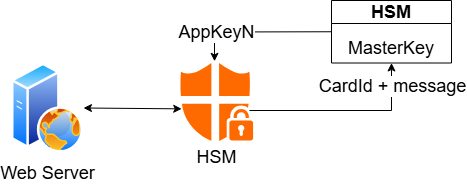
\includegraphics[width=\textwidth]{imaxes/KEY_MANA}
	\caption{Diagrama del sistema de gestión de claves. A la izquierda se representa la memoria de la tarjeta con NDEF y el conjunto protegido de claves, junto con la NACU y el ACMS.}
	\label{fig:key_management}
\end{figure}

\section{Initial prototyping and hardware assembly}
\label{sec:NACU1}

In the initial prototyping phase, the primary objective is to assemble, configure and rigorously validate the hardware components that constitute the access control system using an iterative approach. An Arduino Uno was selected as the main microcontroller to orchestrate sensor and actuator operations, while an ESP32 module provides IEEE 802.11 Wi-Fi and Bluetooth connectivity for bidirectional data exchange with the ACMS \cite{ref45}. NFC functionality is handled by the MFRC522 module, which supports both reading and writing functionalities with NTAG cards.

Seamless interoperability among these devices is essential for establishing a robust, low-latency communication backbone. Accordingly, each component is mounted on a solderless breadboard and interconnected in accordance with the best wiring practices. Comprehensive configuration and functional testing at this stage lay the groundwork for subsequent software integration and the enforcement of cryptographic security protocols.

\subsection{NFC Reader Integration with the Microcontroller}

The MFRC522 module provides two communication interfaces with the Arduino UNO: Serial Peripheral Interface (SPI) and Inter-Integrated Circuit (I2C), operating solely at 3.3 V to guarantee electrical compatibility with the microcontroller. The SPI interface was chosen for this project due to its higher transfer speeds and ease of implementation in prototyping environments.

The physical interconnection was created by soldering the wires according to the following pin diagram (Figure \ref{fig:MFRC-ArduinoUno}):

\begin{table}[H]
	\centering
	\begin{tabular}{|c|c|}
		\hline
		\textbf{MFRC522 PINS} & \textbf{Arduino Uno PINS} \\
		\hline
		3.3V & 3.3V \\
		GND & GND \\
		RST & 9 \\
		SDA & 10 \\
		MOSI & 11 \\
		MISO & 12 \\
		SCK & 13 \\
		\hline
	\end{tabular}
	\caption{MFRC522-Arduino UNO Wiring Following the SPI standard}
	\label{tab:mfrc522_arduino}
\end{table}

\begin{figure}[H]
	\centering
	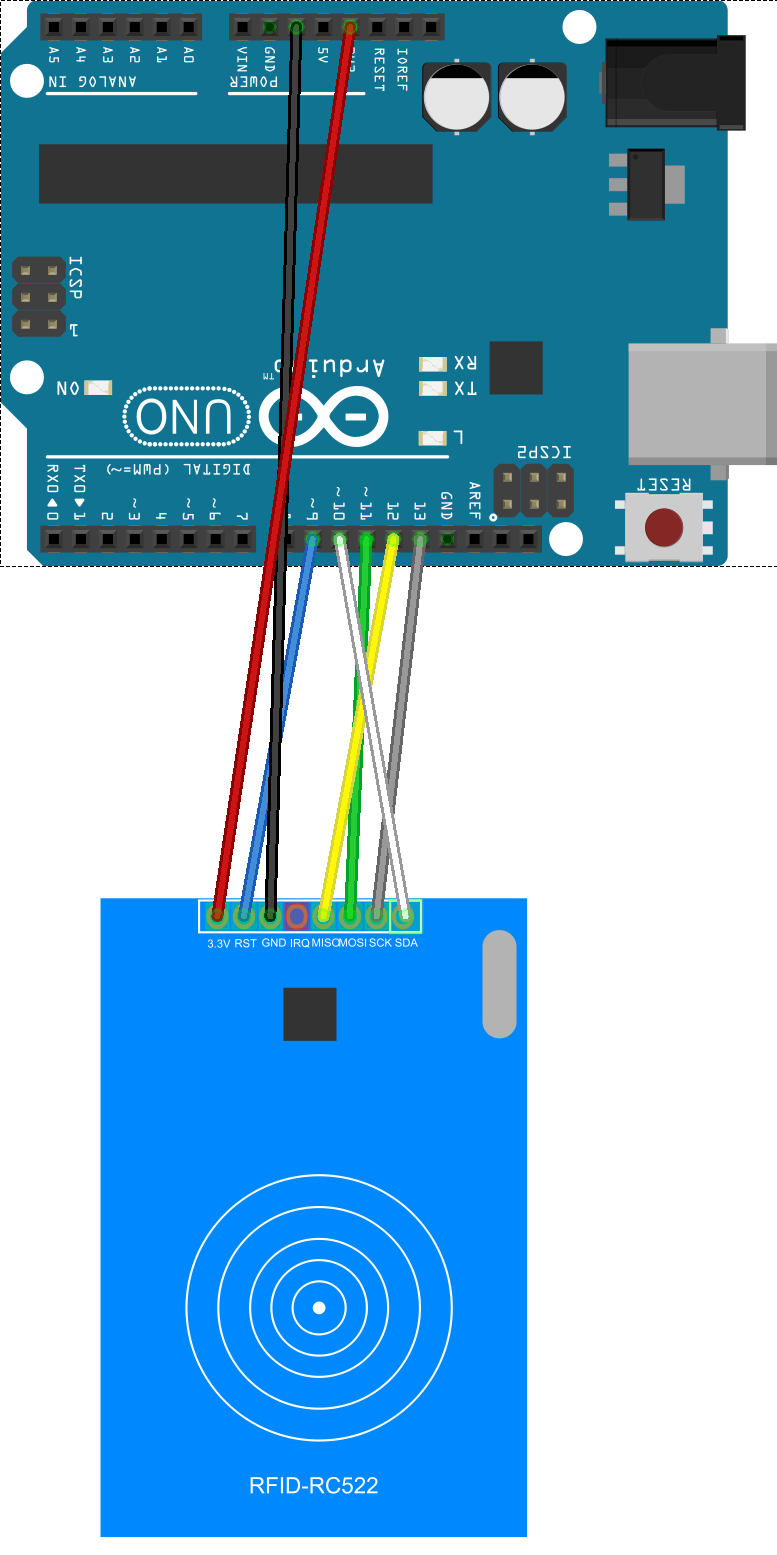
\includegraphics[width=0.5\textwidth]{imaxes/UNOMFRC}
	\caption{MFRC522-ArduinoUNO Wiring Following the SPI standart}
	\label{fig:MFRC-ArduinoUno}
\end{figure}

To validate all cryptographic functionalities of the NTAG424 DNA, the MFRC522\_NTAG424DNA library itself provides a series of test sketches. For each functionality there are three levels of security:

\begin{itemize}
	\item \textbf{PLAIN}: clear text communication.
	\item \textbf{MAC}: adds a message authentication code (MAC) calculated with AES-128, guaranteeing the integrity and authenticity of the commands, but without encrypting the content.
	\item \textbf{FULL}: establishes an end-to-end encrypted channel following an EV2 mutual authentication protocol with AES-128, protecting the confidentiality of all data exchanged \cite{ref42}.
\end{itemize}

\subsection{Wi-Fi module integration}

The ESP32 module provides Wi-Fi and Bluetooth connectivity, forming the bridge between the NFC Access Control Unit (NACU) and the Access Control Management Server (ACMS). To ensure the reliability of the data flow from the Arduino UNO to the ESP32, the serial interconnection is verified before integrating any network logic. The interface chosen is UART (Universal Asynchronous Receiver-Transmitter), due to its wide compatibility, low resource consumption and the need for only two data signals.

It is important to note that the default UART port of the Arduino UNO (pins 0 and 1) is reserved for communication with the computer during sketch loading. Therefore, two additional digital pins and the \texttt{SoftwareSerial} object are used to avoid interference with the USB programmer. Also, the same issue is encountered when configuring this protocol in ESP32, the UART0 (GPIO 1: TX0, GPIO 3: RX0) is reserved for connection to the computer, both for firmware upload and serial monitor, so it should not be used for communication with the Arduino UNO.

Therefore, pin connections are established as follows (Figure \ref{fig:ESP32-ArduinoUno}):

\begin{table}[H]
	\centering
	\begin{tabular}{|c|c|}
		\hline
		\textbf{Arduino UNO pins} & \textbf{ESP32 pins} \\
		\hline
		2 (TX) & 27 (RX) \\
		3 (RX) & 26 (TX) \\
		\hline
	\end{tabular}
	\caption{ESP32-Arduino UNO Wiring Following the UART standard}
	\label{tab:esp32_arduino_uart}
\end{table}

\begin{figure}[H]
	\centering
	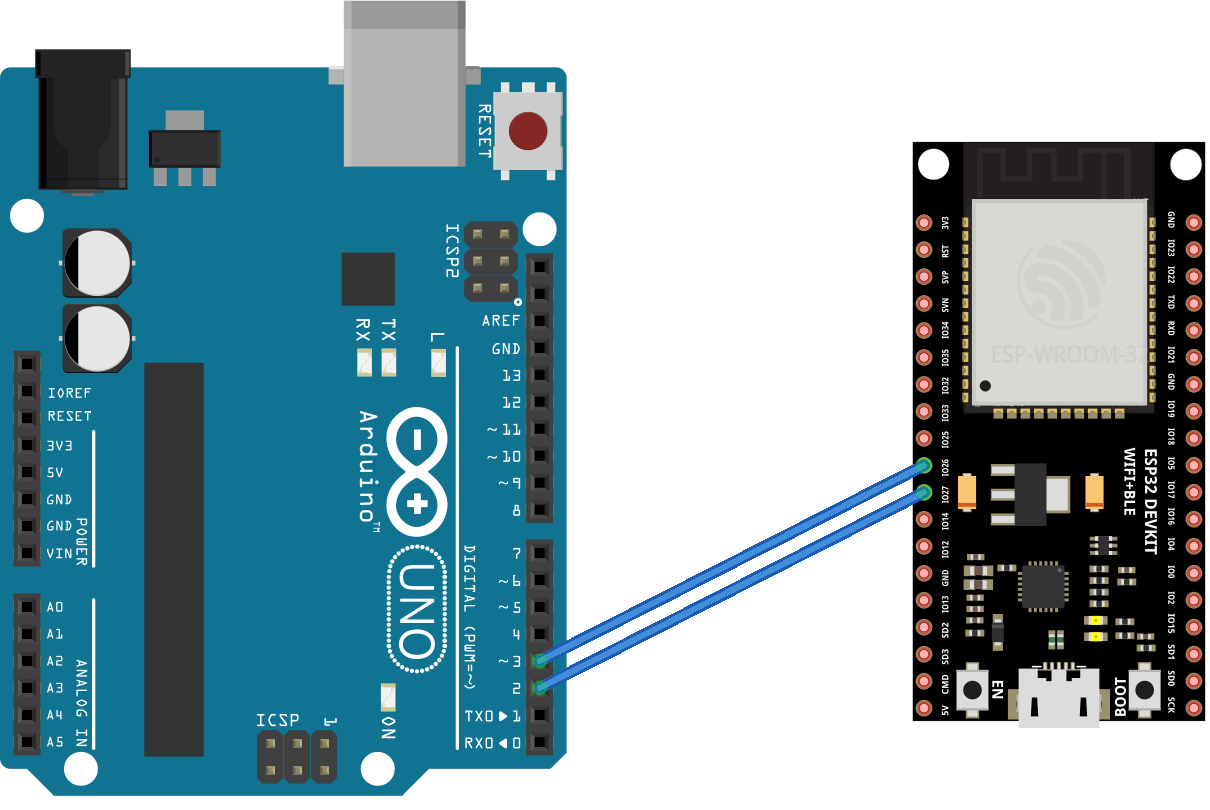
\includegraphics[width=\textwidth]{imaxes/esp32UNO}
	\caption{ESP32-ArduinoUNO Wiring Following the UART standard}
	\label{fig:ESP32-ArduinoUno}
\end{figure}


Each module receives independent power through its connectors, ensuring stability and electrical isolation. Once this UART transport layer is established, access control protocols and HSM commands can be implemented on it without risk of data loss or overlapping.

\subsection{Physical lock integration}


To incorporate the LIBO 12 V/180 kg magnetic lock into the access control prototype, a Dollatek DC 0-5 V relay module is used to interface between the Arduino Uno and the 12 V power supply of the lock (Figure: \ref{fig:maglock_arduino}).

For supplying the relay, 5 V and GND connections from the Arduino Uno are connected to the V\textsubscript{CC} and GND pins of the relay module, respectively. Digital pin DN (configurable in the sketch) goes to the IN pin of the relay.

Also, for powering the lock, the 12 V 1.5 A adapter provides power to the magnetic coil. Its +12 V pole connects to the COM terminal of the relay; the GND of the adapter connects to the return power terminal of the lock.

The NO (Normally Open) terminal of the relay goes to the positive power terminal of the lock. When the relay is activated, it closes the circuit between COM and NO and energizes the coil.

\begin{figure}[H]
	\centering
	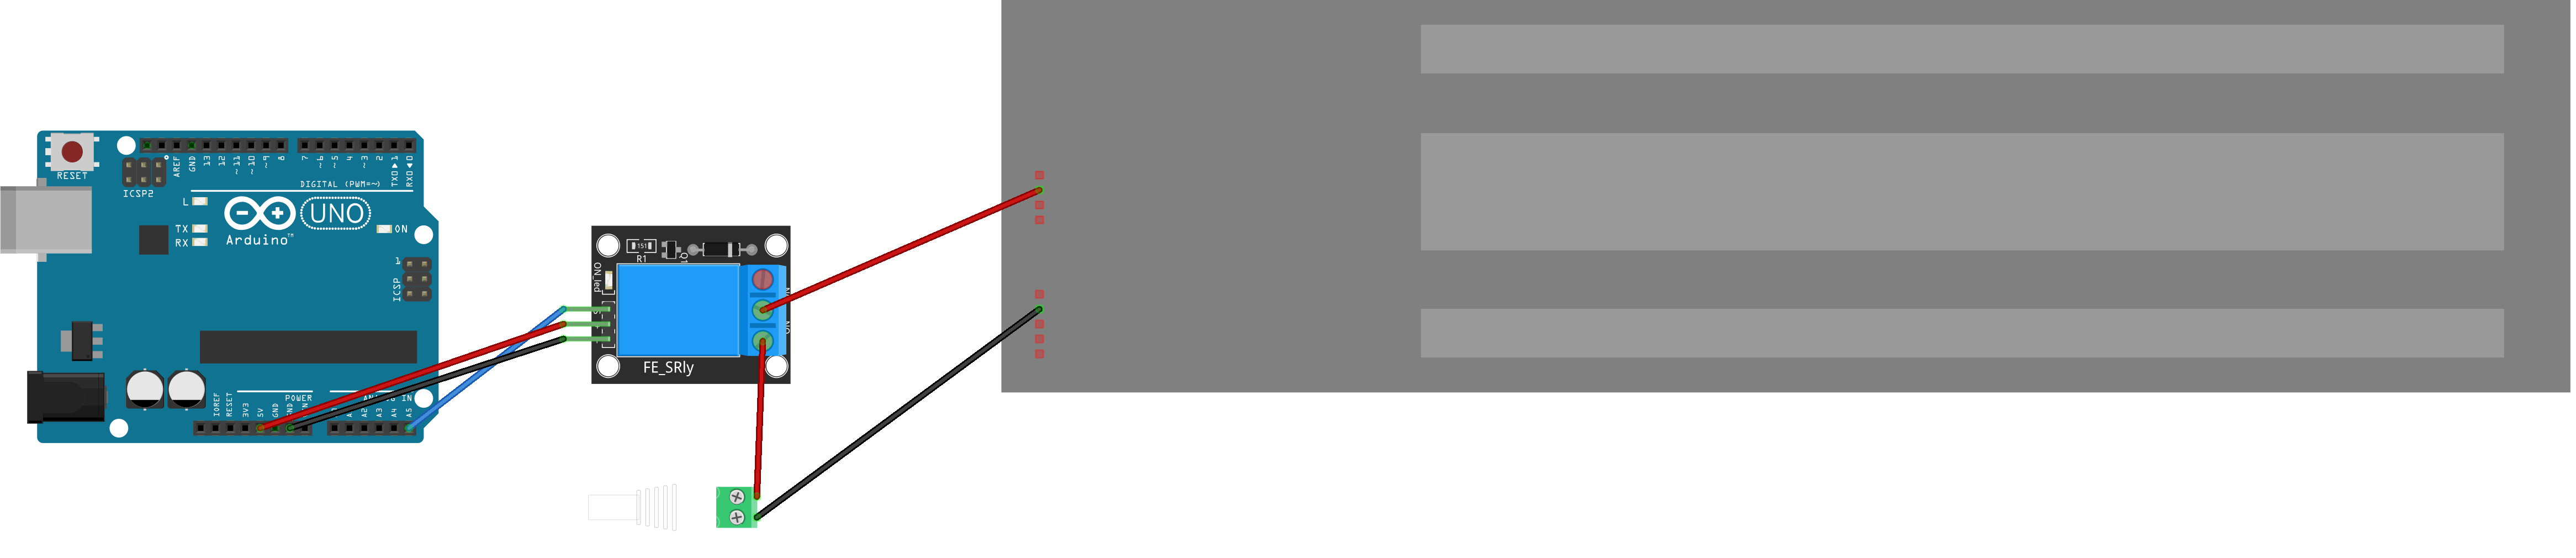
\includegraphics[width=0.7\textwidth]{imaxes/maglock.png}
	\caption{Maglock-Arduino UNO Wiring, with the Arduino connected via 5 V and GND pins for power management to a relay, which obtains power from the voltage adapter to redirect it to the magnetic lock (shown on the right).}
	\label{fig:maglock_arduino}
\end{figure}

\section{NFC Access Control Unit (NACU)}
\label{sec:NACU2}

The objective of this section is to describe how the modular hardware part of the system is created using an iterative scope. In each step, a new module is added and its ability to communicate with the already‑tested modules is verified using the relevant protocol so that by the end of the cycle every hardware element has been proven capable of interoperating reliably under the conditions it will face in the completed system.

\subsection{Iteration 1: Basic NFC communication}

The objective of this iteration is to establish reliable communication between the NFC reader (MFRC522) and the NTAG 424 DNA card, enabling secure extraction of its unique identifier (UID) in “Full” mode (ISO 14443-4) \cite{Ref65}. This iteration lays the foundation for subsequent authentication and key management phases.

Before running any test, the firmware must perform two generic tasks:
\begin{itemize}
	\item The SPI interface is initialized to communicate the microcontroller (Arduino Uno) with the MFRC522 module and the reader performs a software reset.
	\item Each loop verifies that the reader detects a valid card (“OK” status) before proceeding to the next step, thus ensuring that all subsequent operations are performed only when the hardware is ready and the card responds correctly.
\end{itemize}


During this iteration, the wires had to be welded in for the NFC communication to be constant.

\subsubsection{Secure NFC card UID Reading}

In the verification of the NTAG424 DNA UID‐reading functionality, the example sketch \texttt{Full\_GetCardUID} provided by the MFRC522\_NTAG424DNA library is employed as a reference implementation. 

Before each critical operation, the system checks a status code to ensure that the previous step has been completed successfully (“DNA\_STATUS\_OK”). If there is a failure, it returns to the start of the cycle and waits for a card again.

The flow needed to securely read the UID using the library standard is represented in Figure \ref{fig:5.8}:
\begin{enumerate}
	\item The NFC reader identifies that a new card has entered its field and resolves possible collisions to always work with a single tag.
	\item The correct memory area inside the NTAG424 card is accessed for protected operations.
	\item A secure channel via EV2 (Enhanced Version 2) mutual authentication is established using AppKey0.
	\item The 7-byte unique identifier of the card is retrieved under the secure channel, ensuring its confidentiality and integrity.
	\item Finally, the decrypted UID is sent to the serial monitor.
\end{enumerate}

\begin{figure}[htbp]
	\centering
	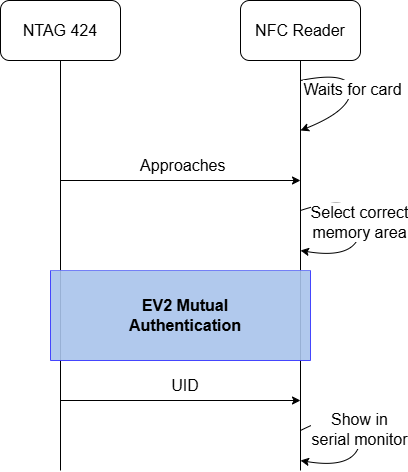
\includegraphics[width=0.6\textwidth]{imaxes/UID_READ} % Añade aquí la ruta de la figura
	\caption{NTAG424 card UID Read after performing mutual authentication with NFC Reader}
	\label{fig:5.8}
\end{figure}

\subsection{Iteration 2: Providing basic Wi-Fi connectivity}

The objective of this iteration is to create a bi-directional, stand-alone communication channel between the Arduino Uno (which manages the NFC reader) and the ESP32 (which connects to the server), without occupying or interfering with the ESP32's USB programming port. This keeps the USB port free for firmware uploads and debugging, while ensuring reliable data exchange between the two microcontrollers.

To ensure proper communication between the computer and the ESP32 module through the Arduino IDE development environment, it is necessary to first proceed with the installation of the corresponding USB-UART driver. In this case, the Silicon Labs CP210x chip is the serial bridge used by most ESP32-based boards, so the “CP210x VCP Drivers” \cite{ref46} driver package must be installed in the operating system. These drivers allow the system to recognize the USB device as a virtual serial port (VCP), enabling program loading and serial monitoring.

Once the driver is installed, the ESP32 is configured within the Arduino IDE. To do it, the official “esp32” plug-in is added in the Board Manager via the URL provided by Espressif Systems. This package includes both the cross-compilation drivers (toolchains) and the libraries necessary for the IDE to detect and program the ESP32 board. After completing this step, any test sketch can be loaded into the module.

In order to test the serial communication between the microcontroller and the WI-FI module, a sketch is uploaded, with the purpose of sending a simple message and displaying it in the serial monitor. In order to perform this task, UART protocol is used via pins RX and TX 2 and 3 in the microcontroller and GPIO 27 and 26 respectively in the WI-FI module. The microcontroller uses the serial bus communication for sending a test message, while the WI-FI module checks whether the channel is free, and then proceeds to listen to it until a space (“\textbackslash n”) is found (Figure \ref{fig:5.9}).

\begin{figure}[htbp]
	\centering
	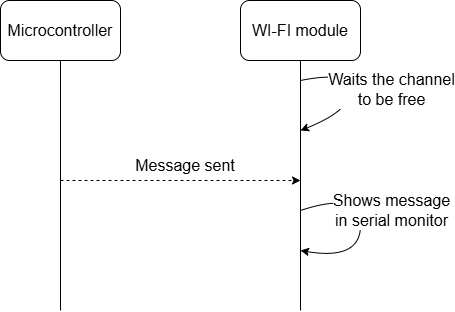
\includegraphics[width=0.6\textwidth]{imaxes/MICROCONTROLLERESP32} % Añade aquí la ruta de la figura
	\caption{ESP32 WI-Fi module Shows UART Message via Serial Monitor}
	\label{fig:5.9}
\end{figure}

\subsection{Iteration 3: Mutual authentication and configuring NFC card identifiers}

The objective of this iteration is to implement EV2 (Enhanced Version 2), which procedure is explained in Section \ref{subsec:EV2}, Full authentication and plain NDEF writing on NTAG424. During this phase, several NTAG424 features are tested, like status error handling, AES-128 handshake, retries on “deselectAndWakeupA” and random challenges generation optimization. Also, writing arbitrary data to the NDEF file raised awareness on the correct setting of offsets and maximum block length for this process to work. In addition, memory cleanup to avoid leaks and buffer management was implemented.

\subsubsection{EV2 Mutual Authentication with AppKey}

The EV2 protocol  in the NACU sketch it is implemented the following way:

\begin{enumerate}
	\item The reader creates a 16‑byte random challenge, RndA, by sampling an entropy source (e.g. \texttt{randomSeed(analogRead(0))} on Arduino) inside the \texttt{generateRndA} function.
	\item It then encrypts RndA with AppKey0 and sends it to the tag to start the EV2 handshake.
	\item The underlying library takes over from there: it receives the tag’s encrypted response, checks that RndA matches the decrypted value (\ref{fig:3.2}), and completes the mutual‑authentication sequence.
\end{enumerate}

\subsubsection{Configuring NFC card identifiers}
\label{subsubsection:cardidload}
To enable uploading card identifiers (CardId) to the NDEF region of the unencrypted NTAG424 DNA card (Plain Mode), the following flow is implemented, inspired by the \texttt{Plain\_WriteData} example in the MFRC522\_NTAG424DNA library, as shown in Figure \ref{fig:5.10}:

\begin{enumerate}
	\item The NFC reader identifies that a new card has entered its field and resolves possible collisions to always work with a single tag.
	\item Then, parameters such as the target file, the position where the data will be written, and the content to be stored are defined.
	\item The serial console printout confirms success or reports the error code (st) in case of failure, allowing to immediately validate if the card stores the NDEF section correctly.
\end{enumerate}

\begin{figure}[htbp]
	\centering
	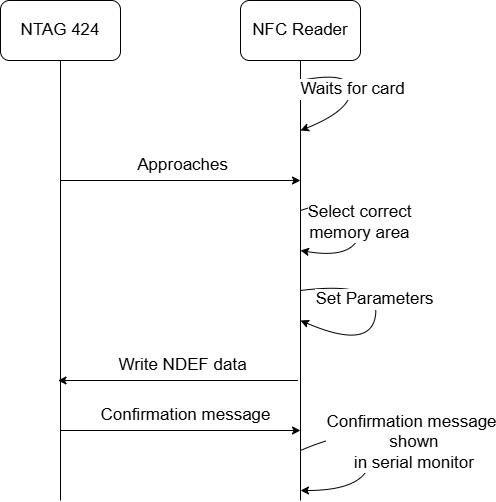
\includegraphics[width=0.6\textwidth]{imaxes/NDEFWIRTE} % Añade aquí la ruta de la figura
	\caption{NTAG 424 NDEF memory file Writing in Plain Mode}
	\label{fig:5.10}
\end{figure}

\subsection{Iteration 4: Reading NFC Card memory and Loading Cryptographic Keys}

The objective of this iteration is to read arbitrary data from the NDEF file and test the key change feature from NTAG424, which is protected by EV2 mutual authentication with the MasterKey.

\subsubsection{Obtaining NFC card identifiers}

One of the fundamental steps to validate system operation is to test the NACU's ability to retrieve data stored on an NTAG424 DNA card. This card has multiple internal files, among which the NDEF (NFC Data Exchange Format) file is commonly used to store structured information readable by NFC compatible devices. In this system, a card identifier is stored in it, and must be retrieved during the personal identification process.

In order to perform basic reading without applying advanced cryptographic authentication, we have chosen to operate in Plain communication mode. This mode allows reading operations to be performed without the need for a prior mutual authentication procedure or channel encryption.

To enable reading data from the NDEF memory region of the NTAG424 DNA on Plain Mode, the following procedure is followed based on the \texttt{Plain\_ReadData} sample sketch from the MFRC522\_NTAG424DNA library, in which after a card is selected and detected(FIgure \ref{fig:5.11}):
\begin{enumerate}
	\item The application designates the NDEF memory area on the card and specifies how many bytes to read.
	\item The NDEF file’s contents are retrieved in clear text and stored in a temporary buffer.
	\item The serial monitor confirms whether the information stored in the buffer is correct.
\end{enumerate}

\begin{figure}[htbp]
	\centering
	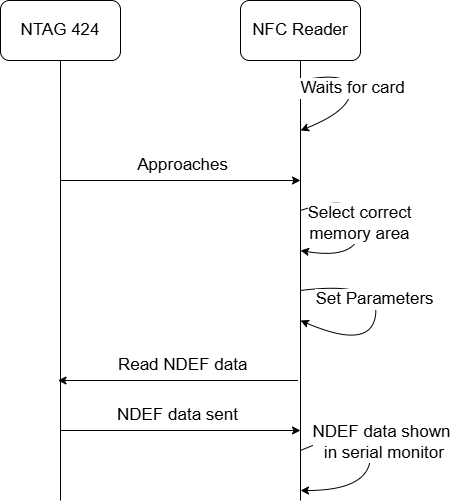
\includegraphics[width=0.6\textwidth]{imaxes/NDEF_READ} % Añade aquí la ruta de la figura
	\caption{NTAG 424 NDEF memory file reading in Plain Mode}
	\label{fig:5.11}
\end{figure}

\subsubsection{Key loading into the NFC card}
\label{subsubsection:keyload}
To securely update any of the keys stored in an NTAG424 DNA it is necessary to use the EV2 protocol (AES-128 mutual authentication) and the \texttt{DNA\_Full\_ChangeKey} function of the MFRC522\_NTAG424DNA library as shown in Figure \ref{fig:5.12}:
\begin{enumerate}
	\item The MasterKey is used in the EV2 mutual authentication.
	\item Then, a new key is defined using:
	\begin{enumerate}
		\item \texttt{keyNumberToChange} selects the AppKey to be used as the target of the update.
		\item \texttt{newKey} as the 16-byte array with the desired new value.
		\item \texttt{newKeyVersion}, a byte that increments the internal version, allowing to manage key versions.
	\end{enumerate}
	\item Finally, the key is changed using the \texttt{DNA\_Full\_ChangeKey} function and validated through the serial monitor.
\end{enumerate}

\begin{figure}[H]
	\centering
	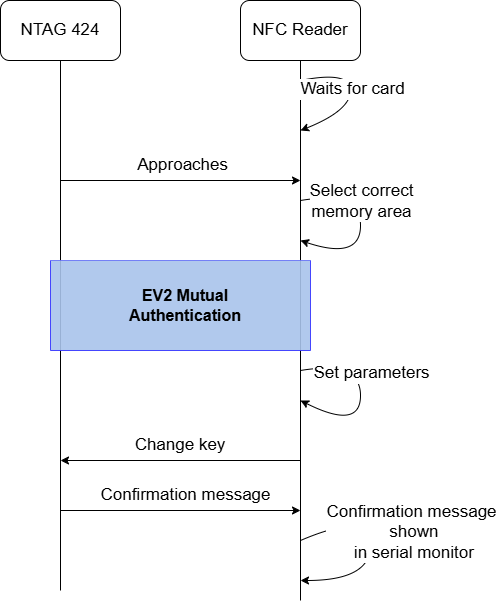
\includegraphics[width=0.6\textwidth]{imaxes/KEYCANGE} % Añade aquí la ruta de la figura
	\caption{Change of NFC NTAG424 card AppKey1, which needs EV2 mutual authentication}
	\label{fig:5.12}
\end{figure}

\subsection{Iteration 5: NACU Subsystem Full Integration}

The objective of this iteration is to connect UID reading with ESP32, for later sending the UID to the ACMS. In order to achieve it, sketches must be consolidated, elaboration of single flow with test scripts of Wi-Fi module and microcontroller. To validate the end-to-end flow, NFC reader obtains the UID of a NTAG424 card, microcontroller sends it over UART and WI-FI module checks its arrival via serial monitor.

\subsubsection{Card UID and AES Key Transfer between NACU modules}

To verify the UART data flow that is used in the final product, the UID of an NTAG424 DNA card is read in “plain” (unencrypted) mode and forwarded by the microcontroller by the UART port to the WI-FI module, which receives it and displays it on the screen as in the previous test. In this way, we verify that the board identifier is reliably transmitted along the system (Figure \ref{fig:5.13}).

\begin{figure}[htbp]
	\centering
	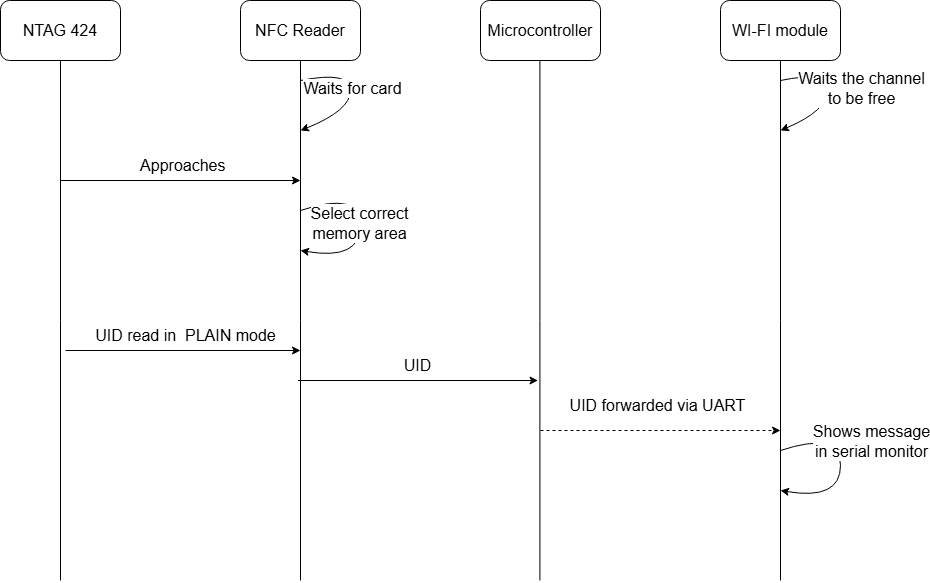
\includegraphics[width=\textwidth]{imaxes/FINALFLOW} % Añade aquí la ruta de la figura
	\caption{ESP32 Wi-FI module receiving via UART NTAG 424 UID after plain read performed by the NFC Reader}
	\label{fig:5.13}
\end{figure}

Also, in order to validate the transmission of fixed-length binary data backwards, the Wi-FI module sends via UART an AES-128 key (AppKey) as a 16-byte array. On the microcontroller, a sketch similar to the one for receiving the UID is executed: it reads exactly 16 bytes from the serial port, displays them on the monitor and uses this key to perform mutual authentication in a compatible card using the NFC reader. 


\subsection{Iteration 6: Magnetic lock Management for Physical Access Control}

The objective of this iteration is to implement the logic to integrate the Maglock in the system. This component only needs to communicate with the Arduino Uno, which must control the voltage in order to manage the unlocking of the Maglock when needed.

For performing this action, one analog pin from the Arduino Uno must be connected to the relay, and in the \texttt{setup()} part of the code its voltage must be set to HIGH in order to lock it. Then, when the situation is needed, the voltage of this pin must be set to LOW in order to unlock it.


\section{Access Control Management Server (ACMS)}
\label{sec:ACMS}

The objective of this section is to create a backend administration server using an incremental approach. The Django~\cite{Ref20} framework was chosen for this task because the Model‑View‑Controller~\cite{Ref61} architecture, combined with a built-in admin and login interface provides the scalability, security, and rapid‑development capabilities best suited to the project needs.

\subsection{Iteration 1: Basic Structure and Authentication}

The objective of this iteration is to provide the ACMS with a strong basis by implementing a RESTful API and a robust authentication system. These foundations will allow, in successive iterations, to incrementally incorporate the specific functionalities needed to complete the entire access control flow.

\subsubsection{Time Window Based Access Control and Auditory}

First, an internal application called \texttt{core} was created to encapsulate all the specific logic for access control and communication with the NFC Access Control Unit (NACU). Django follows the Model-View-Template (MVT) pattern, so the first step was to define the models that would represent the domain entities in the data layer. All of them were declared in \texttt{core/models.py} and registered in the administration panel through \texttt{core/admin.py}, which facilitates the management of users, schedules and keys directly from the Django Admin interface. The most relevant model classes were:

\begin{itemize}
	\item \textbf{HSMData}: Stores personal data associated with the user and the card UID linked to him.
	\item \textbf{AccessLog}: Logs each access attempt, storing the UID sent, the user's name (related to the corresponding entry in HSMData) and the timestamp of the event. In addition, an \texttt{authorized} boolean field was included indicating whether access was granted according to the configured schedule.
	\item \textbf{EntrySchedule}: Allows defining the valid access time slots for each user, linked to the HSMData entity.
\end{itemize}

Once these models were defined, the framework's own migrations were executed with the \texttt{makemigrations} and \texttt{migrate} commands, synchronizing the definition of the tables in the database.

To provide visual consistency and facilitate the reuse of components in template-based views, a global template folder was set up in \texttt{settings.py} using the line \texttt{'DIRS': [BASE\_DIR / 'templates']}. From here, a base file (\texttt{base.html}) was implemented to serve as a common template for all views, and specific templates \texttt{login.html} and \texttt{log\_list.html} were generated to extend \texttt{base.html} to cover the different functionalities of the system. As for the views and routes layer, the fundamental REST endpoints were defined in \texttt{core/views.py} (Figure~\ref{fig:mvc-schema}).

\begin{figure}[H]
	\centering
	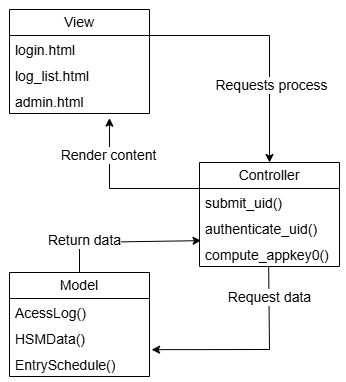
\includegraphics[width=0.75\textwidth]{imaxes/MVC.png}
	\caption{MVC Schema Representing the Views, that are managed by the Controller, that extracts data from the Model}
	\label{fig:mvc-schema}
\end{figure}

\subsubsection{Access Control Endpoints for Administration and NACU Communication}

In this section the three HTTP endpoints that form the core API between the NFC access control units (NACU) and the Access Control Management Server (ACMS) are defined. Together they handle every card‐based access attempt, recording each try, validating against registered UIDs and time schedules, and automating alerts, while also providing an interface for administrators.

\begin{itemize}
	\item \textbf{/submit\_uid/ (POST/GET)}
	\begin{itemize}
		\item Receives the NFC card UID.
		\item Immediately saves an attempt record.
		\item Checks if the UID exists and, if it does, validates if it is within its authorized schedule.
		\item Updates the log with the result and, if not allowed, triggers a mail alert.
	\end{itemize}
	
	\item \textbf{/authenticate\_uid/ (GET)}
	\begin{itemize}
		\item Verifies the existence and schedule of the UID.
		\item Logs the result.
		\item Redirects to view where all access logs are displayed.
	\end{itemize}
	
	\item \textbf{/log\_list/ (GET)}
	\begin{itemize}
		\item Retrieves all logs.
		\item Renders the view for administrators to review.
	\end{itemize}
\end{itemize}

\subsection{Iteration 2: Key Derivation System}

In this second iteration, the objective is to deploy and configure a Hardware Security Module (HSM) in software, and to create in the ACMS an endpoint that, from a \texttt{CardId} and a \texttt{message}, generates the \texttt{AppKey0} key using HMAC-SHA256.

\subsubsection{Hardware Security Module Implementation}

In the system, the Master Key plays a key role in terms of security. It is not only used to load the AppKeys on each card, but also to derive all subsequent keys. Its compromise compromises the confidentiality of the entire infrastructure. For this reason, the Master Key must be given a higher level of protection than any other cryptographic credential.

For development and test environments, SoftHSM is used, a software-based HSM implementation that complies with the PKCS\#11~\cite{Ref76} specification. A slot in PKCS\#11 is a logical container that can hold a token. Before we can store keys, we must create and initialize that token on disk and assign it an administrator PIN (SO-PIN) and a user PIN. After uploading two different keys into the slot, the result is shown in Figure~\ref{fig:hsm-slots}.

\begin{figure}[H]
	\centering
	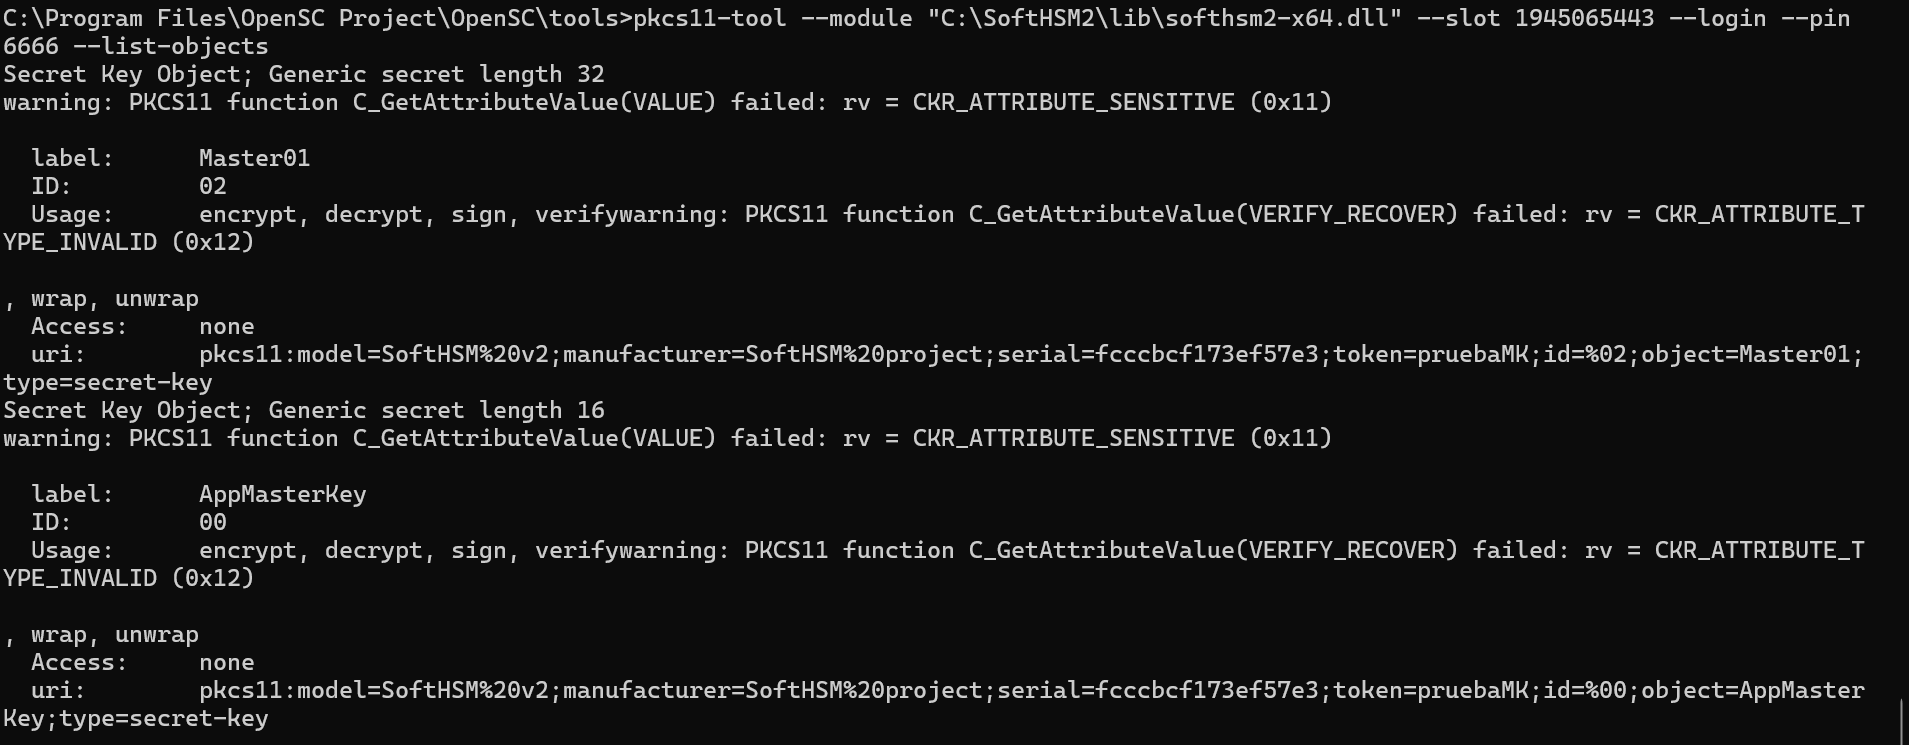
\includegraphics[width=\textwidth]{imaxes/hsm.png}
	\caption{Slots of HSM. Master01 and AppMasterKey are stored and labeled, with no access allowed and the type of object is secret-key}
	\label{fig:hsm-slots}
\end{figure}

\subsubsection{Key Derivation System Integration in ACMS}

To invoke the virtual HSM from Django, the \texttt{/compute\_appkey0/} endpoint dumps the concatenation \texttt{cardid\_bytes + msg} to disk and, via a subprocess invoking the same command used in CMD, requests the SoftHSM2 token to execute an HMAC-SHA256 with the Master Key. The PKCS\#11 module signs the input file and deposits the result in \texttt{OUTPUT\_PATH}. Django then opens this file, extracts the first 16 bytes of the HMAC and returns them as a hexadecimal string.

\subsubsection{Key Derivation Endpoint}

The purpose of the endpoint \texttt{/compute\_appkey0/} (GET) is to derive a 128-bit key (AppKey0) using HMAC-SHA256 on the \texttt{CardId} and a contextual message.

\textbf{Parameters:}
\begin{itemize}
	\item \texttt{CardId}: card identifier in hexadecimal (32 hex digits).
	\item \texttt{msg}: additional text string to be concatenated to the identifier.
\end{itemize}

\textbf{Main flow:}
\begin{enumerate}
	\item Validates presence of \texttt{CardId} and \texttt{msg}, returns 400 if missing.
	\item Converts \texttt{CardId} to bytes, returns 400 if format invalid.
	\item Concatenates bytes and writes to input file.
	\item Invokes \texttt{pkcs11-tool.exe} externally. Raises 500 on failure.
	\item Reads HMAC result and checks length.
	\item Extracts first 16 bytes and returns them as uppercase hex string.
\end{enumerate}


The endpoint uses \texttt{@csrf\_exempt} so NACU can call it directly. Any error returns HTTP 500 for immediate reader-side detection.


\subsection{Iteration 3: Transport encryption (HTTPS/TLS)}
\label{subsec:https}

The objective of this iteration is to increase the security of the ACMS for it to scale from HTTP, which is the default from Django, to HTTPS/TLS.

\subsubsection{ACMS Communication Encryption}

In order to guarantee the confidentiality and integrity of communications between the NACU and the Django server during the development phases, the server was scaled from HTTP to HTTPS using locally trusted self-signed certificates.

Django's \texttt{runserver} default command only exposes HTTP (no encryption). \texttt{Django-sslserver} \cite{Ref47} is a development extension that enables a temporary HTTPS server, suitable for local environments. Its use in production environments is not recommended, but it is ideal for end-to-end TLS verification in development.

\texttt{Mkcert} \cite{Ref48} is the command-line utility chosen to generate "locally trusted" X.509 certificates. It installs a private Certificate Authority (CA) in the operating system's certificate store, allowing you to quickly create valid TLS certificates for local IP addresses or domains without browser security warnings.

Also, in order to establish TLS/SSL connections from the NACU, Arduino IDE provides the \texttt{WiFiClientSecure} \cite{Ref49} library. It supports the encryption and negotiation process of the TLS protocol and can accept self-signed certificates if configured with \texttt{setInsecure()}. In addition, the \texttt{HTTPClient} \cite{Ref50} library is provided to facilitate making HTTP(S) requests over a \texttt{WiFiClient} or \texttt{WiFiClientSecure}.

\textbf{General flow:}
\begin{enumerate}
	\item Installation of the local CA. With Mkcert a Certificate Authority is created and imported into the system's certificate store. From then on, any certificate issued by that CA will be recognized as valid by the OS and local browsers.
	\item X.509 TLS \cite{Ref77} certificates are issued for the IP address (or hostname) of the Django server, along with its private key.
	\item Django configuration. Django-sslserver is added to the application.
	\item The list of allowed hosts (\texttt{ALLOWED\_HOSTS}) is updated to include the IP of the server and ESP32.
	\item Launch of the development server under HTTPS, pointing to the certificate and its key generated with Mkcert.
	\item In the Wi-Fi module firmware, \texttt{WiFiClientSecure} is used to establish TLS connections.
\end{enumerate}

Furthermore, the ACMS development instance is launched in HTTPS mode, via the \texttt{django-sslserver} extension, by specifying the TLS certificate (\texttt{certs/IP.pem}) and its corresponding private key (\texttt{certs/IP-key.pem}). This ensures that all incoming requests are handled over an encrypted channel.

\subsection{Iteration 4: Real Time Access Control Mail Alert System}
\label{subsec:email}

The objective of this iteration is the integration of an immediate notification mechanism, which is essential in an access control system, as it allows the administrator to be alerted to critical events. In the case of this system, unauthorized access attempts in real time, enabling corrective action to be taken as quickly as possible.

From the perspective of notification system design, it is common to consider two main modes: synchronous notification and asynchronous notification. In the synchronous model, the Django view that handles the HTTPS request is directly responsible for invoking the mail sending via the \texttt{django.core.mail.send\_mail()} function before formulating the response to the client. This approach guarantees absolute immediacy in the generation of the alert, since the administrator receives the mail almost simultaneously with the registration of the incident on the server. However, the main disadvantage lies in the fact that the API response time may be affected by the latency of the SMTP server.

A secure SMTP configuration is essential. The STARTTLS protocol (port 587) makes it possible to initiate the connection in plain text and then negotiate the TLS layer, so that both the credentials and the message content are encrypted along the way \cite{Ref78}. When using email accounts from providers such as Gmail, it is advisable to generate "App Passwords", especially when the primary user has multi-factor authentication.

\subsubsection{Mail Alert System Implementation in Django}

The mail sending logic is integrated directly into the \texttt{submit\_uid} view-in charge of processing each access attempt-so that, after evaluating the authorization conditions, the \texttt{send\_mail()} function is invoked in those cases where the authorization is denied. The Django configuration to enable the SMTP backend is done in \texttt{settings.py}.

There is no need to modify \texttt{INSTALLED\_APPS}, since the SMTP backend is natively built into Django. Thanks to the \texttt{EMAIL\_USE\_TLS=True} directive, the STARTTLS layer is automatically enabled, protecting credentials and email content.

Also, the \texttt{send\_mail()} function creates and sends the message in the same thread that processes the request, so notification is almost immediate. By using the \texttt{fail\_silently} parameter, it is guaranteed that if the SMTP server does not answer or returns an error, the access request will continue to be processed without interruption to the client.

\subsection{Iteration 5: Role-Based Access Control}
\label{subsec:roles}

The objective of this iteration is to create a prototype with a minimum of profile-based access control. In order to develop it, a \texttt{Role} model has been added that is associated one by one with each \texttt{HSMData} record, both defined in the \texttt{models.py} file. Thus, when creating or editing a user in the Django admin panel, the admin can directly assign a role (e.g. \texttt{admin}, \texttt{employee}, \texttt{guest}). In \texttt{admin.py} Roles can be added.

To identify which NACU makes the request (necessary in scenarios with multiple access points), an auxiliary function has been implemented in \texttt{views.py} that parses the message received at the key derivation endpoint (\texttt{compute\_appkey0}). This message takes the form \texttt{GETUIDN}, where \texttt{N} is the reader identifier. The function extracts this digit by regular expression.

When invoked before processing the \texttt{AppKey0} derivation, \texttt{parse\_reader\_number} allows recording in the internal log which device originated the request and, in a full deployment, to condition the authorization not only on the time but also on the user profile and the reading terminal.

For now this role and reader detection logic serves to demonstrate the feasibility of the approach: in production it would be extended to validate fine-grained permissions (e.g. "only users of role 'admin' can enter through reader 2"). In this academic phase it is sufficient to record both values and show how they could be integrated into authorization decision making.

\section{Full System Integration \\ \& Testing}

The full system integration aims to verify that all system components, from the NACU and the hardware module to the ACMS and the HSM, work in a coordinated manner and meet the security, reliability and performance requirements defined in the project. In this phase, the complete data flow, as conceived in the architectural design, is assembled and subjected to several tests that simulate real life situations. This is the final architecture of the system, which will be used in this simulation:

For these tests, three users were defined in the model with different allowed schedules (see Table~\ref{tab:test-users}):

\begin{table}[H]
	\centering
	\begin{tabular}{|c|c|c|}
		\hline
		\textbf{USER} & \textbf{NFC UID} & \textbf{SCHEDULE} \\
		\hline
		USER1 & 04440DCA9C1790 & 18PM--6AM \\
		\hline
		USER2 & 044A85CA9C1790 & 6AM--18PM \\
		\hline
		USER3 & 044A78CA9C1790 & 9AM--14PM \\
		\hline
	\end{tabular}
	\caption{Test Users Definition with UID and schedule}
	\label{tab:test-users}
\end{table}

As for this academic demo, only one reader is used, so roles were not defined for these users because all the petitions come from the very same device.

\begin{figure}[H]
	\centering
	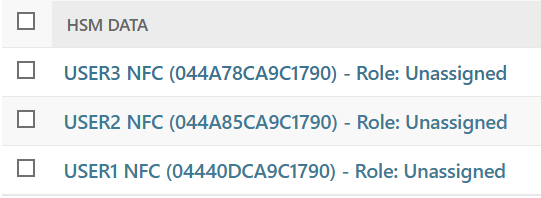
\includegraphics[width=0.9\textwidth]{imaxes/Tests_Users.png}
	\caption{Test Users (1--3) Creation without Role assignation}
	\label{fig:test-users}
\end{figure}

Several CardIDs were first programmed into each card’s NDEF memory using the corresponding modified microcontroller sketch (~\ref{subsubsection:cardidload}). With the MasterKey already loaded into the HSM, the \texttt{/compute\_appkey0/} endpoint was called, sending the message \texttt{READUID1} to derive each card’s AppKey0. Finally, the \texttt{FULL\_ChangeKey} sketch was run on the microcontroller, which authenticates with the MasterKey using the NFC reader and replaces the default card key with the freshly derived AppKey0. After these steps, all cards are fully provisioned and ready for secure operation.

Then, the process defined in the personal authentication data flow (Figure \ref{fig:Personal Auth Data Flow}) starts:
\begin{enumerate}
	\item The USER2 card is approached to the NFC Access Control Unit (NACU) and its NDEF (CardId) file is read (Figure \ref{fig:ndef-read}).
\end{enumerate}

\begin{figure}[H]
	\centering
	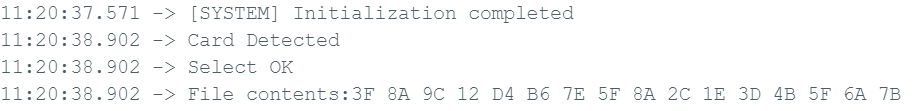
\includegraphics[width=0.9\textwidth]{imaxes/CARDIDREAD}
	\caption{NDEF File Read Integration}
	\label{fig:ndef-read}
\end{figure}

\begin{enumerate}
	\setcounter{enumi}{1}
	\item After the CardId is obtained, it is sent to the ACMS \texttt{/compute\_appkey0/} endpoint through the Wi-Fi module, along with the \texttt{READUID1} message.
	\item AppKey0 is returned to the Wi-Fi module and sent to the microcontroller.
	\item Mutual authentication is performed to read the UID (Figure \ref{fig:mutual-auth}).
\end{enumerate}

\begin{figure}[H]
	\centering
	\includegraphics[width=0.75\textwidth]{imaxes/mutualauth_UID}
	\caption{Mutual Authentication in the Final System}
	\label{fig:mutual-auth}
\end{figure}

\begin{enumerate}
	\setcounter{enumi}{4}
	\item The UID is sent to the \texttt{/submit/} endpoint of the ACMS through the Wi-Fi module.
	\item An authorization message is returned and sent to the microcontroller with a code: 0 for access denied and 1 for access allowed.
	\item The message confirms that the access is denied and the magnetic lock remains locked.
	\item Finally, a mail is sent to the administrator informing of the unauthorized access attempt (Figure \ref{fig:denied-mail}).
\end{enumerate}

\begin{figure}[H]
	\centering
	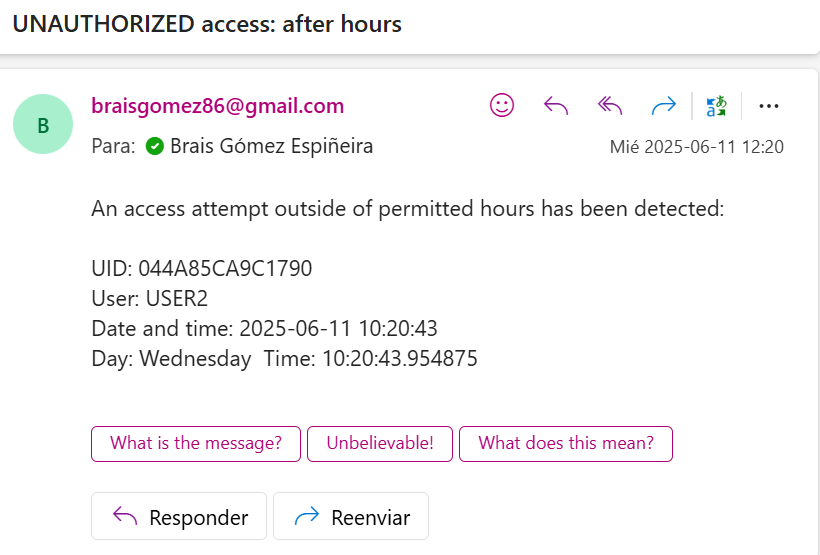
\includegraphics[width=0.75\textwidth]{imaxes/Correo_denegado}
	\caption{Mail Acknowledging Denied Access}
	\label{fig:denied-mail}
\end{figure}
\begin{figure}[H]
	\centering
	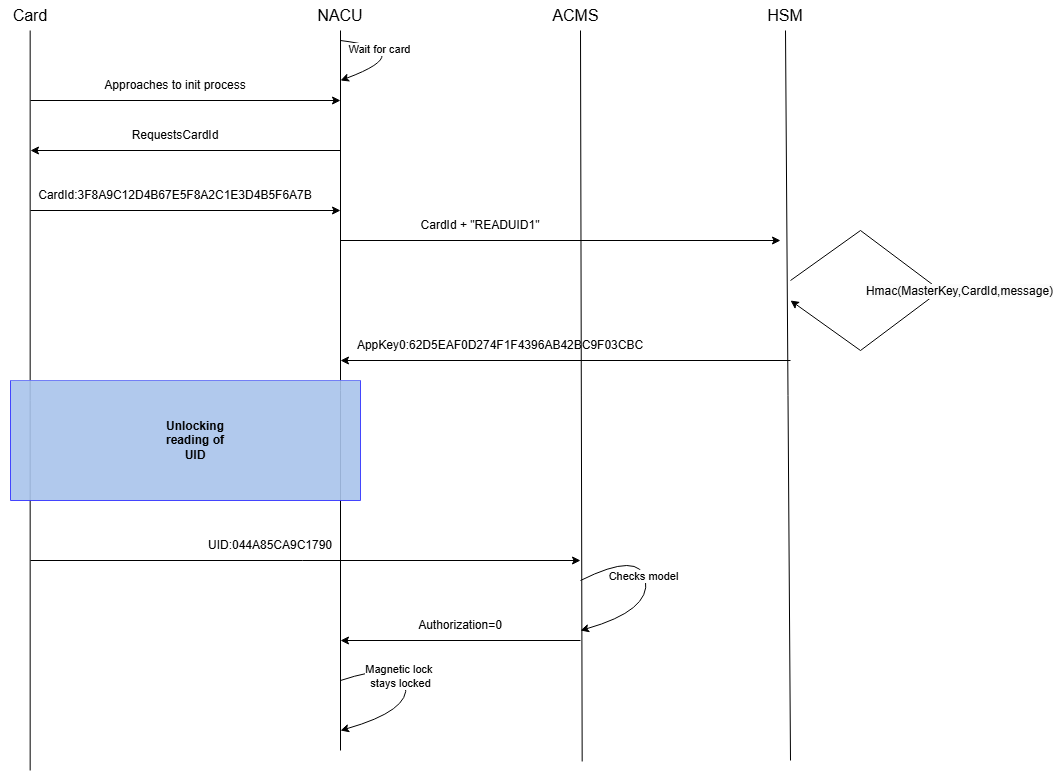
\includegraphics[width=0.75\textwidth]{imaxes/TIDF}
	\caption{Personal authentication data flow for the test case}
	\label{fig:Personal Auth Data Flow}
\end{figure}

USER2 is out of its allowed schedule, which means that the lock does not unlock. Then, the exact same process is repeated with USER1, which is on its allowed schedule, and the lock allows the access as shown in Figure \ref{fig:uid-ok}.

\begin{figure}[H]
	\centering
	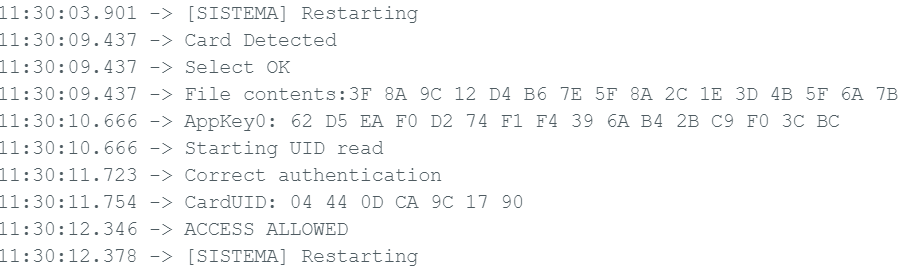
\includegraphics[width=0.9\textwidth]{imaxes/User_Allowed}
	\caption{USER1 Access Allowed Arduino Uno Serial Monitor Data Flow}
	\label{fig:uid-ok}
\end{figure}

\section{Threat Analysis}
\label{sec:threat_analysis}

This project is deeply focused on security, providing confidentiality, authenticity and integrity in identification systems, mitigating threats inherent to the technologies used and IoT environments.

Regarding NFC~\cite{Ref54}, one of the main threats is eavesdropping. Communication between two devices over an NFC channel can be intercepted using several devices such as Flipper Zero or Proxmark 3~\cite{Ref55}, which are designed to exploit vulnerabilities in systems that use ISO 14443A NFC. Although the required physical proximity (less than 10 cm) limits the attack, the use of high-gain antennas or resonant couplings can extend the effective range.

Another risk, related to eavesdropping, is cloning or tag impersonation, which consists in an attacker uploading a stolen NFC tag in another device such as ChameleonMini \cite{Ref57}, trying to impersonate its legit owner. Thanks to mutual authentication, none of these attacks are effective in this system: an attacker could obtain the \texttt{CardId}, but this does not compromise the user nor the whole system. Without access to the HSM it is impossible to derive \texttt{AppKey0}.

There are also interference and denial of service (DoS) attacks that can affect this type of systems. Generating electromagnetic noise in the NFC band or saturating the reader with multiple requests can cause failures or crashes. However, using maglocks ensures that this attack would not let the attacker pass through the protected door. This is because voltage is constantly supplied to the lock, and in order to open it, a voltage cut-off is needed. If the reader were to be saturated, the door would not open because the reader itself would not be able to send the voltage cut-off signal.

In addition, one of the main physical threats is the manipulation of the wiring between Arduino and ESP32, which could lead to data leaks. As this system is designed for academic purposes, wiring is not protected. If this system needs to be installed in a real environment, a proper safe box must be used in order not to be easily manipulated. It is also important to highlight that no key is stored in any of these microcontrollers, as it is considered a malpractice.

Related to the Access Control Management Server (ACMS), several attacks including SQL Injection, XSS in the API, TLS certificate theft, and DoS against the server could be performed. To mitigate these threats, the information that is stored in the Django model database is not critical or personal (e.g., NIF or keys). The NFC tag is stored in it but, again, in case of compromise, it would not be enough to authenticate in the system. Moreover, the \texttt{MasterKey} is stored in a Hardware Security Module to prevent these types of attacks from being effective.


 \chapter{Results and Discussion}
\label{chap:results}

This project achieved an open, modular and cost-effective solution for NFC access control, capable of securely and reliably managing locks electronically and recording events. After all the project objectives were met, this chapter describes the qualitative results obtained after the implementation and validation of the system.

\section{NFC Access Control Unit (NACU)}
\label{sec:nacu}

The NACU, see \ref{sec:NACU1} \& \ref{sec:NACU2}, was developed with an iterative approach, adding and validating each hardware module sequentially to ensure their correct communication and joint operation. The following hardware modules form the NACU (Figure~\ref{fig:nacu_hardware}): 
\begin{itemize}
	\item MFRC522 reader: NFC reader compatible with NTAG424 and that supports AES-128 encryption.
	\item Arduino UNO: microcontroller that encapsulates the logic of the NACU.
	\item Magnetic lock: physically controls access from the voltage signals received from the microcontroller.
	\item ESP32: Wi-Fi module that provides connectivity with the ACMS.
\end{itemize}

Using an iterative approach, each hardware module was integrated and tested one by one with those already implemented, to form a single unit capable of:
\begin{itemize}
	\item UID protected reading via EV2 (Enhanced version 2) mutual authentication.
	\item NDEF memory reading and writing.
	\item Key changing using master key.
	\item UID and AES-128 key forwarding between embedded components.
	\item Ability to create HTTPS petitions to REST API, communicating with Access Management Control Server (ACMS) via Wi-Fi.
	\item Capacity to lock/unlock a magnetic lock in order to control physical access.
\end{itemize}

\begin{figure}[h]
	\centering
	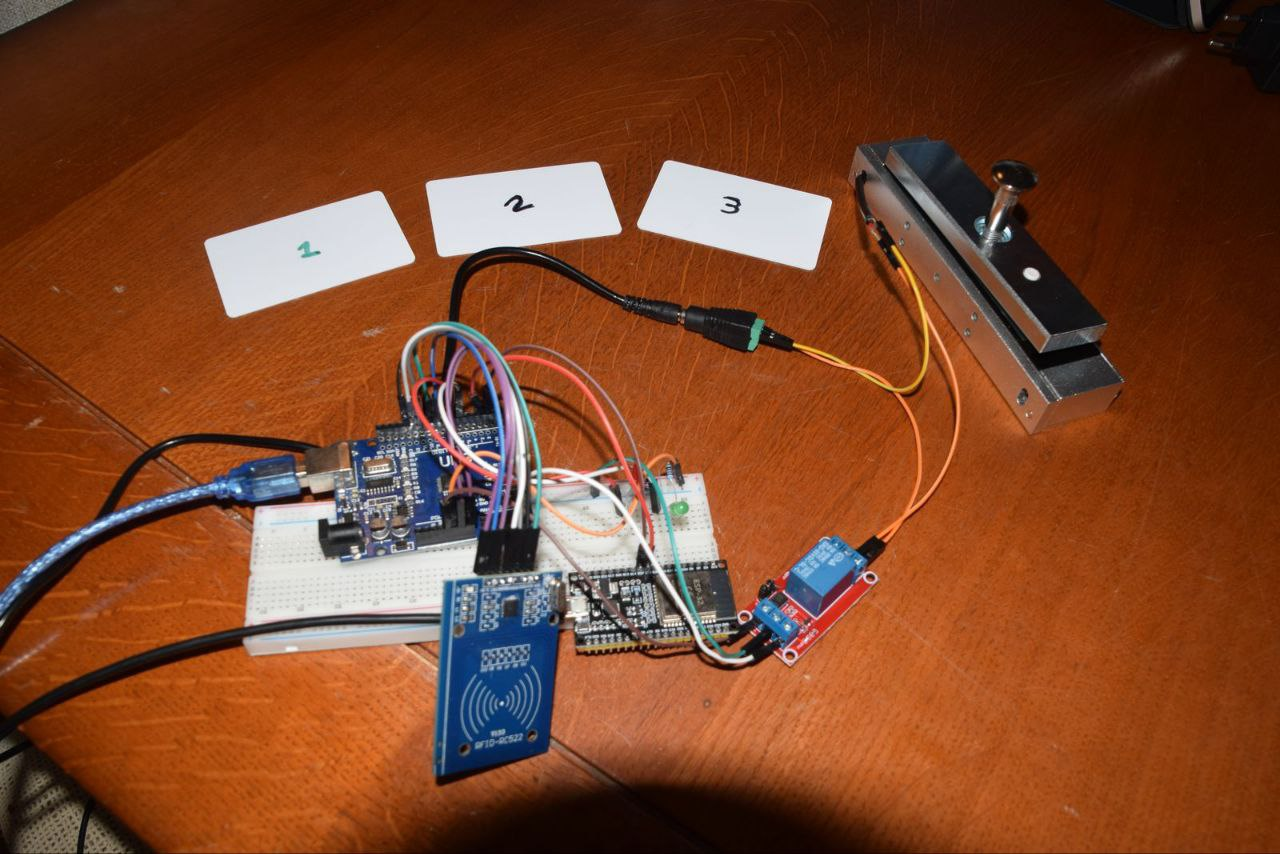
\includegraphics[width=0.8\textwidth]{imaxes/NACU} % Inserta aquí la imagen real si la tienes
	\caption{NACU and Test Cards. From left to right, the Arduino Uno, MFRC522, ESP32 and magnetic lock can be seen. Also, the three cards at the back are the ones used to test the system.}
	\label{fig:nacu_hardware}
\end{figure}

\section{Access Control Management Server (ACMS)}
\label{sec:acms}

As a result of the incremental development of ACMS, a complete system with the following functional capabilities was obtained:
\begin{itemize}
	\item User and role management: adding and deleting users with permissions assignment.
	\item Credential control: loading and protection of master keys in the simulated HSM and AppKey derivation.
	\item Access validation: reception of NACU requests, UID and time window checking, and allow or deny access control.
	\item Real-time auditing: detailed log of each entry attempt.
	\item Alert system: immediate email notification in case of unauthorized access.
	\item Administrative interface: web views to view access logs, manage schedules, review and revoke credentials.
\end{itemize}

The ACMS, \ref{sec:ACMS}, was implemented in Django following an incremental methodology. In the first phase the REST API base was created, and in the following phases security, management and presentation functionalities were added until completing a server capable of processing all NACU access trial requests. The architecture, shown in Figure~\ref{fig:acms_architecture}, combines a Django server over HTTPS/TLS, with its own default model database, with a software Hardware Security Module (HSM) implementation (SoftHSM/PKCS\#11) to protect cryptographic keys.

\begin{figure}[h]
	\centering
	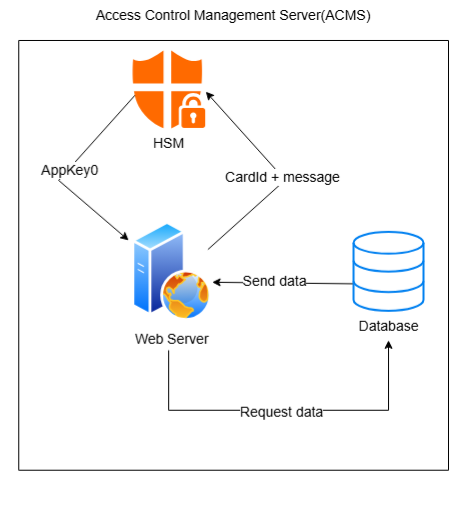
\includegraphics[width=0.8\textwidth]{imaxes/ACMS} % Inserta aquí la imagen real si la tienes
	\caption{ACMS Architecture Scheme including HSM, the web server and the default Django model database}
	\label{fig:acms_architecture}
\end{figure}

This architecture is able to perform the following protocols in order to process NACU requests:
\begin{itemize}
	\item Key derivation via HMAC-SHA256 in the HSM, so that the NACU can request the key needed for reading the card UID and it can be successfully obtained without storing it in a vulnerable database or exposing the master key.
	\item NFC personal UID validation on ACMS, managing time-based access control.
\end{itemize}

Also, an administration interface was defined using the default views offered by Django, including a login view (Figure~\ref{fig:login_view}) and an administration panel for data modeling. In addition, a log list view (Figure~\ref{fig:log_list_view}) was created for the administrator to be able to check all the access attempts into the physical facility that the access control system is protecting. By displaying both successful and failed attempts, this view gives administrators a clear audit trail to spot unusual patterns, investigate security incidents, verify policy compliance and fine-tune access rules over time.

\begin{figure}[h]
	\centering
	\includegraphics[width=0.8\textwidth]{imaxes/login} 
	\caption{Administration Default Login system}
	\label{fig:login_view}
\end{figure}

\begin{figure}[H]
	\centering
	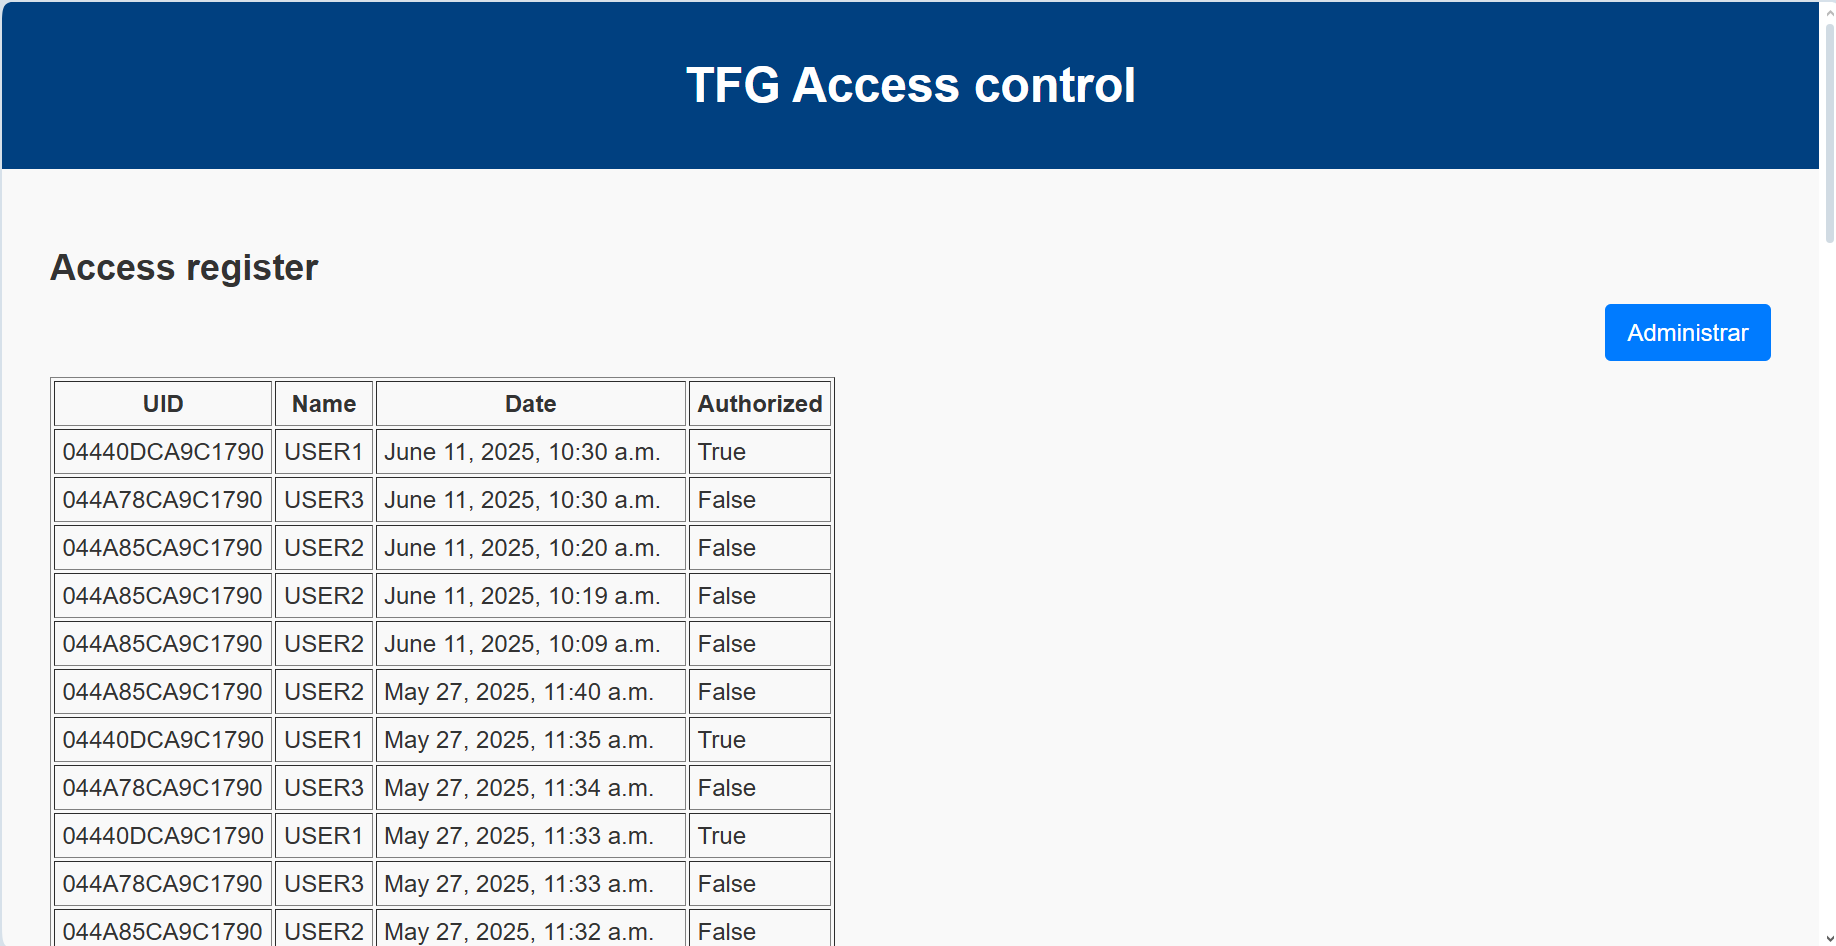
\includegraphics[width=0.8\textwidth]{imaxes/loglist} % Inserta aquí la imagen real si la tienes
	\caption{Log List Administration View}
	\label{fig:log_list_view}
\end{figure}

\clearpage

\subsection{Defined Endpoints}
The endpoints defined for this project are presented below. The ACMS code is completely open-source and is organized in a modular way, so that new functionalities can be easily incorporated on this already implemented base.

\begin{table}[H]

	\begin{tabular}{|l|l|p{2.5cm}|p{2.5cm}|}
		\hline
		\textbf{Endpoint} & \textbf{Method} & \textbf{Request payload} & \textbf{Response Payload} \\ \hline
		/submit\_uid/ & GET & uid (hexadecimal string, required) & JSON \{ message, uid, timestamp, authorized[, error] \} \\ \hline
		/authenticate\_uid/ & GET & uid (hexadecimal string, required) & Redirect to log\_list view (HTML with log list) \\ \hline
		/log\_list/ & GET & --- & HTML rendering of core/log\_list.html with logs \\ \hline
		/compute\_appkey0/ & GET & cardid (hex), msg (string) & JSON (pure) with hex string of 32 chars or error JSON \\ \hline
	\end{tabular}
	\caption{ACMS Endpoints Overview}
	\label{tab:endpoints}
\end{table}

\section{Key Management and Security System}
In this system, a software-based Hardware Security Module (SoftHSM) was built and integrated into the ACMS authentication server to safeguard all critical cryptographic material. Rather than relying on Django’s default key handling, SoftHSM, a software HSM implementation (PKCS\#11-compatible), was implemented to store the Master Key securely and derive per-card AppKey0 values via HMAC-SHA256. An ACMS endpoint receives a cardId and a msg, forwards them to the HSM for secure key derivation, and returns only the resulting AppKey0, ensuring that neither the Master Key nor any intermediate secrets ever leave the protected HSM environment. This custom HSM integration follows the key management architecture laid out in \ref{subsec:keymanagement} (Figure~\ref{fig:key_management}).

\begin{figure}[h]
	\centering
	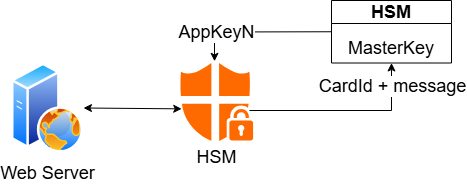
\includegraphics[width=0.7\textwidth]{imaxes/KEY_MANA} % Inserta aquí la imagen real si la tienes
	\caption{Key Management System in the HSM}
	\label{fig:key_management}
\end{figure}

For protecting the master key:
\begin{itemize}
	\item A token is initialized using SoftHSM, creating a secure disk slot protected by an administrator PIN and user PIN.
	\item The Master Key is loaded into the token, making it impossible to retrieve in clear text.
\end{itemize}

Then, the endpoint /compute\_appkey0/ was created to derive AppKey0 via HMAC-SHA256 from a cardId and a msg, using the Master Key without ever exposing it. Protecting the Master Key is critical; its compromise would endanger the confidentiality of every derived key and, ultimately, the security of the entire system.

\section{Access Control System Secure Communications}
To ensure the confidentiality and integrity of communications between the NACUs and the ACMS server, in the third iteration of the incremental development of it (\ref{subsec:https}), the channel was changed from HTTP to HTTPS/TLS in the development environment. Django-sslserver was integrated to enable TLS on the Django server and Mkcert was used to generate a local Certificate Authority that issues X.509 certificates trusted by the operating system and browsers. On the Wi-Fi module, the WiFiClientSecure library was used to establish TLS connections, configured to accept Mkcert's self-signed certificates. Thanks to this setup, all REST requests are end-to-end encrypted, ensuring that both credentials and sensitive data travel securely without validation errors or local security warnings.

\section{Role-based Access Control Management}
As explained in \ref{subsec:roles}, the system was extended with basic profile-based access control and multi-reader identification. This feature allows administrators to tailor entry permissions per user group; granting, for example, employees access to internal offices while restricting guests to reception areas, thus managing who can open which doors in a multi-reader deployment simply by assigning roles.

A new Role model was linked one-to-one with HSMData, allowing administrators in the Django panel to assign roles (e.g., “admin”, “employee”, “guest”), as shown in Figure~\ref{fig:role_management}, directly when creating or editing users. To distinguish between multiple NACU units, a helper was implemented in views.py to parse the reader ID messages of the form “GETUIDN” at the /compute\_appkey0/ endpoint. This process enables the log to capture both the user’s role and the originating reader, demonstrating how future production logic could enforce fine-grained rules (for example, “only admins may use reader 2”). In this prototype phase, recording these values suffices to validate the feasibility of integrating roles and reader detection into the authorization workflow.

\begin{figure}[h]
	\centering
	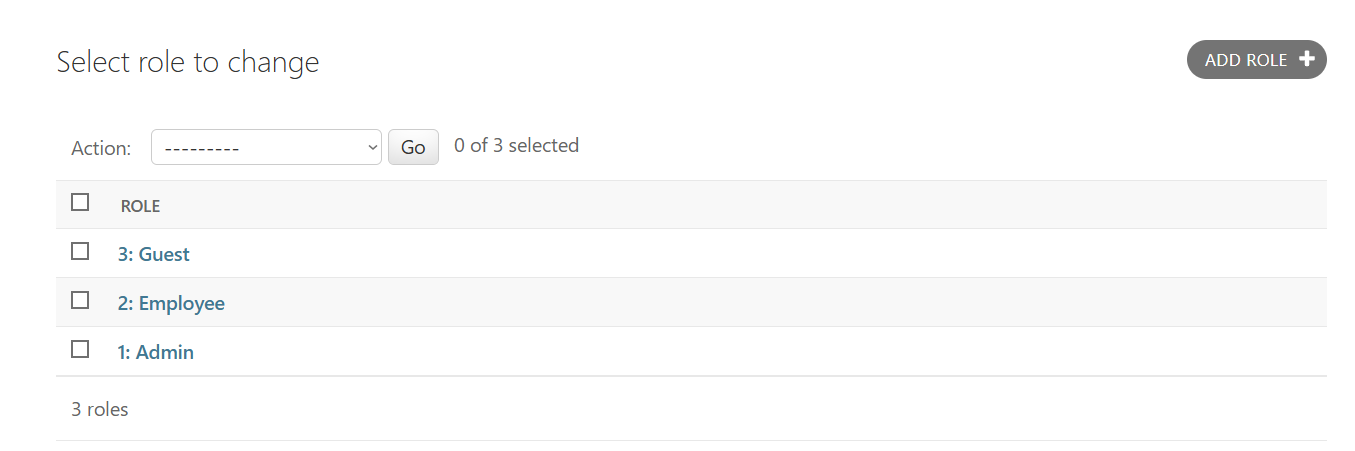
\includegraphics[width=0.7\textwidth]{imaxes/Roles} % Inserta aquí la imagen real si la tienes
	\caption{Role Management view}
	\label{fig:role_management}
\end{figure}

\section{Real-time Unauthorized Access Attempt Alert System}
Real-time email notifications enable a company to detect and respond immediately to security incidents, reducing the window of vulnerability, improving compliance with audit requirements, and minimizing the risk of unauthorized entry. In this forth iteration, as explained in \ref{subsec:email}, immediate email notifications for unauthorized access attempts were integrated directly into the /submit\_uid/ view. Using Django’s built-in SMTP backend, configured to work with TLS and STARTTLS on port 587, the system encrypts credentials and message content end-to-end. Also, to balance immediacy and reliability, alerts are sent synchronously, ensuring the administrator is notified as soon as an incident is logged, while the \texttt{fail\_silently} option is set to True in order to prevent SMTP errors from disrupting the access-control flow. This prototype demonstrates a robust, low-overhead mechanism for real-time monitoring of critical events.

\begin{figure}[h]
	\centering
	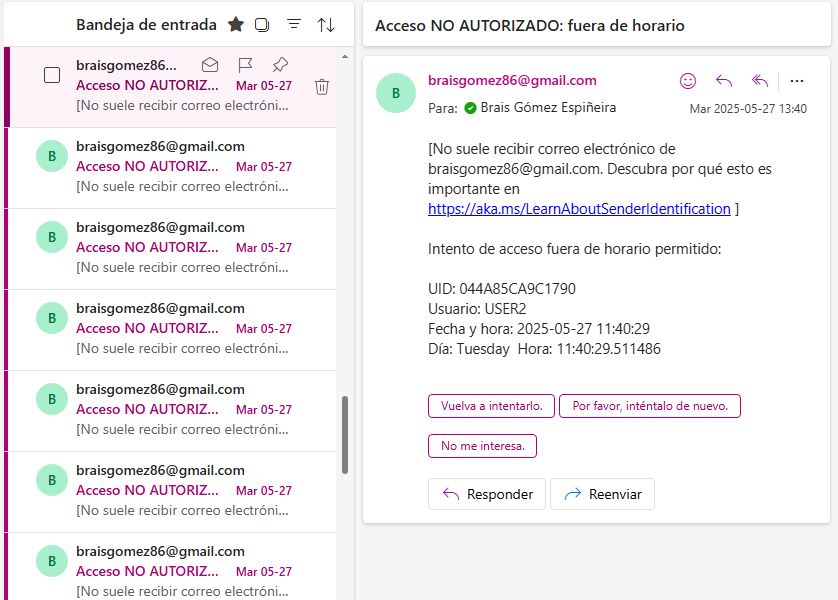
\includegraphics[width=0.7\textwidth]{imaxes/MAIL} % Inserta aquí la imagen real si la tienes
	\caption{Unauthorized Mails Example}
	\label{fig:unauthorized_mail}
\end{figure}


%\include{contido/...}
 \chapter{Conclusions and Future Research}
\label{chap:conclusions}
The development and integration of an NFC-based secure access control system presents a number of complex challenges spanning hardware, firmware and backend services. The implementation of mutual authentication with ISO 14443 A (EV2) and AppKey0 derivation using HMAC-SHA256 in a hardware security module has proven effective in ensuring the confidentiality, authenticity and integrity of CardId and UID exchanges. The modular architecture of the system ,consisting of an Arduino, ESP32 and MFRC522 NFC Access Control Unit(NACU), a Django REST API and a SoftHSM2 HSM (or equivalent), facilitates a clear separation of concerns, simplifies maintenance and allows testing of individual components in isolation. 

Also, the prototype’s academic orientation leaves several practical aspects unaddressed, notably physical protection of wiring, deployment automation (e.g., with containers or orchestration) and comprehensive side‑channel resistance. Moreover, while SoftHSM2 emulates production HSM behavior, real hardware modules may exhibit different performance and security characteristics, which warrants further validation.

\section{Future Research}
\label{sec:future_research}
Several research lines can be followed in order to expand the functionalities, security and performance of the system:

\begin{itemize}
	\item \textbf{Physical and Embedded Hardening.} Investigate the design of a rugged, shielded enclosure that protects both the reader and the UART connections between Arduino and ESP32. This would include tamper-evidence scans and intrusion sensors, as well as the use of microcontrollers with secure enclaves such as TrustZone~\cite{Ref56}.
	
	\item \textbf{Integration with Mobile Apps and Biometrics.} Extend the NFC flow to incorporate an additional biometric-based authentication factor (fingerprint or facial recognition) through a mobile app, exploring APIs such as Android BiometricPrompt~\cite{Ref57}.
	
	\item \textbf{Automated Deployment and Orchestration.} Dockerize the ACMS to facilitate deployment in production environments, including setting up secure networks on AWS and continuous integration (CI/CD)~\cite{Ref58}.
	
	\item \textbf{Evolution to Commercial HSM Hardware.} Replace SoftHSM2 with certified HSM modules and measure actual throughput, latency and power consumption metrics. Compare their resilience against side-channel attacks and TLS certificate validation.
	
	\item \textbf{Dynamic Credential and KeyWheel Support.} Investigate hot AppKey0 and MasterKey key rotation schemes, as well as transitive or delegated credentials, for scenarios where multiple systems must validate the same card without sharing the master key.
	
	\item \textbf{Anomaly Detection and Machine Learning.} Develop behavioral analysis modules based on machine learning that monitor access patterns (read rate, time locations) and alert on unusual attempts or advanced relay attacks~\cite{Ref59}.
\end{itemize}

 %%%%%%%%%%%%%%%%%%%%%%%%%%%%%%%%%%%%%%%%
 % Apéndices, glosarios e bibliografía  %
 %%%%%%%%%%%%%%%%%%%%%%%%%%%%%%%%%%%%%%%%

 \appendix
 \appendixpage
 \chapter{Material adicional}
\label{chap:adicional}



%\include{anexos/...}

 \printglossary[type=\acronymtype,title=\nomeglosarioacronimos]
 \printglossary[title=\nomeglosariotermos]

 \bibliographystyle{IEEEtranN}
 \bibliography{\bibconfig,bibliografia/bibliografia}
 \clearpage
 
\end{document}

%%%%%%%%%%%%%%%%%%%%%%%%%%%%%%%%%%%%%%%%%%%%%%%%%%%%%%%%%%%%%%%%%%%%%%%%%%%%%%%%
